\documentclass{sn-preview}
%% Springer Nature LaTeX template (sn-jnl). Reference style: sn-mathphys-num (numbered).
\usepackage{graphicx}
\usepackage{multirow}
\usepackage{amsmath,amssymb,amsfonts}
\usepackage{booktabs}
\usepackage{array,tabularx}
\usepackage{xurl}
\usepackage{textcomp}
\usepackage{xcolor}
\usepackage{newunicodechar}
\providecommand{\pandocbounded}[1]{#1}
\newunicodechar{≥}{\ensuremath{\geq}}
\newunicodechar{≤}{\ensuremath{\leq}}
\newunicodechar{±}{\ensuremath{\pm}}
\newunicodechar{×}{\ensuremath{\times}}
\newunicodechar{−}{\ensuremath{-}}
\newunicodechar{→}{\ensuremath{\rightarrow}}
\newunicodechar{≈}{\ensuremath{\approx}}
\newunicodechar{∼}{\ensuremath{\sim}}
\newunicodechar{∈}{\ensuremath{\in}}
\newunicodechar{λ}{\ensuremath{\lambda}}
\newunicodechar{σ}{\ensuremath{\sigma}}
\newunicodechar{π}{\ensuremath{\pi}}
\newunicodechar{Σ}{\ensuremath{\Sigma}}
\newunicodechar{·}{\ensuremath{\cdot}}
\newunicodechar{₂}{\textsubscript{2}}
\newunicodechar{₃}{\textsubscript{3}}
\newunicodechar{⁻}{\textsuperscript{\ensuremath{-}}}
\newunicodechar{¹}{\textsuperscript{1}}
\newunicodechar{²}{\textsuperscript{2}}
\newunicodechar{³}{\textsuperscript{3}}
\newunicodechar{⁴}{\textsuperscript{4}}
\newunicodechar{⁺}{\textsuperscript{+}}
\newunicodechar{–}{--}
\newunicodechar{—}{---}
\newunicodechar{‘}{`}
\newunicodechar{’}{'}
\newunicodechar{“}{``}
\newunicodechar{”}{''}
\newunicodechar{ä}{\"a}
\newunicodechar{ö}{\"o}
\newunicodechar{ü}{\"u}
\newunicodechar{é}{\'e}
\newunicodechar{č}{\v{c}}
\newunicodechar{í}{\'\i{}}
\newunicodechar{α}{\ensuremath{\alpha}}
\newunicodechar{μ}{\ensuremath{\mu}}
\newunicodechar{Δ}{\ensuremath{\Delta}}
\newunicodechar{√}{\ensuremath{\surd}}
\newunicodechar{∞}{\ensuremath{\infty}}
\newunicodechar{⁰}{\textsuperscript{0}}
\newunicodechar{₀}{\textsubscript{0}}
\newunicodechar{₁}{\textsubscript{1}}
\newunicodechar{ }{\,}
\newunicodechar{ }{~}
\newunicodechar{…}{\ldots{}}
\newunicodechar{Å}{\AA{}}

\raggedbottom

\begin{document}

\title[Spectrum-native proteomics benchmark]{From identification-first to spectrum-native proteomics: a ground-truth benchmark with real-data validation}

\author*[1]{\fnm{M.} \sur{Nisha Angeline}}\email{nishavlsidesign@gmail.com}

\affil*[1]{\orgdiv{Department of Electronics and Communication Engineering}, \orgname{Velalar College of Engineering and Technology}, \orgaddress{\street{Thindal}, \city{Erode}, \postcode{638012}, \state{Tamil Nadu}, \country{India}}}

\abstract{Mass-spectrometry proteomics is shifting from identification-first workflows, in which tandem (MS2) spectra are matched to a sequence database before any statistics are done, to spectrum-native models that learn directly from MS1 and MS2 signal. Because the ground truth of real spectra is itself defined by identification, how much information identification discards has been hard to quantify. We built an open, CPU-trainable virtual instrument with exact ground truth and used it to benchmark database search, a spectrum-graph algorithm and SpecNovo, a transformer for database-free sequencing, together with identification-first and identification-free phenotype classifiers, including a ProFormer-style transformer with self-supervised pretraining. A differentiable fragment-ion-evidence term raised SpecNovo peptide recall from 0.5\% to 41.6\%. Unlike database search, SpecNovo recovered variant and novel-proteome peptides (38.9\% and 38.7\%) and gave the best-calibrated confidence. Removing identification was the dominant effect for phenotype prediction (AUROC 0.975 vs 0.648 when half of the biomarkers were unidentifiable), whereas pretraining mainly improved transfer to unseen acquisition sites (0.728 vs 0.651). Validation on PRIDE-derived LC-MS/MS runs and MassIVE-KB spectra confirmed the bottleneck: only 0.19\% of 25,613 real MS1 features were identified at 1\% FDR. Calibrating the simulator to measured fragmentation statistics doubled SpecNovo's real-spectrum peptide recall from 7.6\% to 15.1\%, matching a spectrum-graph baseline in precision--coverage AUC. Spectrum-native learning recovers signal that identification-first pipelines lose, but at current data scales it depends on physics-informed inductive biases and on calibration to real instruments.}

\keywords{De novo peptide sequencing, Transformer, Spectrum-to-phenotype, Self-supervised learning, Mass spectrometry, Benchmark}

\maketitle

\section{Introduction}\label{sec:intro}
Mass-spectrometry (MS)-based proteomics has, for two decades, followed an \emph{identification-first} paradigm: tandem (MS2) spectra are matched to peptide sequences drawn from a protein database, matches are filtered by target--decoy competition at a fixed false-discovery rate (FDR), identified peptides are rolled up to proteins, and only then is the resulting quantitative matrix handed to statistics or machine learning \cite{aebersold2016,cox2008,elias2007}. The paradigm is mature and well controlled, but it is lossy by construction. In typical data-dependent acquisition (DDA) experiments, a majority of acquired MS2 spectra remain unassigned; peptides carrying single amino-acid variants (SAAVs), unanticipated post-translational modifications (PTMs), non-canonical open reading frames or organisms absent from the database are invisible; and the stochastic sampling of precursors for fragmentation produces missing values that are neither missing completely at random nor easy to impute \cite{lazar2016,mann2021}. Every downstream biological conclusion therefore inherits the blind spots of the identification step.

Two developments are now loosening this constraint. First, public repositories have grown into corpora of hundreds of millions of spectra (e.g., PRIDE and MassIVE-KB) \cite{perez2022,wang2018}, and are being curated into machine-learning-ready datasets in the spirit of ``MassNet-style'' corpora that can be consumed without bespoke search pipelines. Second, transformer architectures \cite{vaswani2017} have proved able to learn directly from the irregular, set-structured signal of mass spectra. Transformer-based \emph{de novo} sequencing --- Casanovo \cite{yilmaz2024}, InstaNovo \cite{eloff2025}, π-HelixNovo \cite{yang2024}, NovoB \cite{lee2024}, pairwise-attention encoders \cite{lapin2025} and DIA-specific variants \cite{ebrahimi2023} --- translates peaks into peptides without a database, building on the earlier deep-learning de novo work of DeepNovo \cite{tran2017} and PointNovo \cite{qiao2021}. In parallel, ProFormer \cite{krull2026} showed that a transformer operating on MS1-level peptide-ion features can classify single-cell and plasma proteomes by phenotype \emph{without} peptide identification, outperforming conventional machine learning and image-based convolutional networks; a related proteomics transformer (Proformer) \cite{qiu2025} predicts multi-disease risk from large plasma cohorts. Spectrum representation learning (GLEAMS \cite{bittremieux2022}) and fragment-intensity prediction (Prosit, AlphaPeptDeep) \cite{gessulat2019,zeng2022} complete the picture of a field moving from ``identify peptides, then do statistics'' to ``learn directly from MS1/MS2 signal''.

This shift raises questions that are difficult to answer on public data alone, because the ground truth of real spectra is itself defined by identification pipelines. \emph{How much information is lost by identification-first workflows, and under what conditions? When does a database-free model beat a database search, and when does it not? Does self-supervised pretraining on unlabeled runs --- the core premise of corpus-scale ``proteomics GPTs'' --- translate into label efficiency for phenotype prediction? And are spectrum-native models interpretable at the level of individual fragment ions or peptide features?}

Here we address these questions with a fully controlled, open-source \emph{virtual instrument}: a physics-informed simulator of MS2 fragmentation and LC-MS1 acquisition with known ground truth, combined with CPU-trainable transformer models and strong classical baselines. Our contributions are:

\begin{enumerate}
\def\labelenumi{\arabic{enumi}.}
\item
  \textbf{An open benchmark environment} (Python/PyTorch, CPU-only) generating 250,000 labelled MS2 spectra from a 3,000-protein training proteome, ten held-out test sets that vary database membership, fragment completeness and chemical noise, and multi-site LC-MS1 cohorts in which a controllable fraction of biomarkers is \emph{unidentifiable} by MS2 search.
\item
  \textbf{SpecNovo}, an encoder--decoder transformer for database-free sequencing with three inductive biases --- complementary-ion peak encoding, prefix-mass-conditioned decoding and a differentiable ion-evidence term --- whose contributions are quantified in an ablation study.
\item
  \textbf{FeatureFormer}, a ProFormer-style transformer over identification-free MS1 feature tokens, pretrained with masked-intensity modelling on unlabeled runs, benchmarked against identification-first, match-between-runs (MBR) and identification-free linear pipelines across label budgets, unseen acquisition sites and a ``dark-proteome'' sweep.
\item
  \textbf{Quantitative interpretability}: peak-level gradient × input attribution for de novo sequencing and feature-level attribution for biomarker recovery, together with replicate-retrieval analysis of learned spectrum embeddings.
\item
  \textbf{Real-data validation} on PRIDE-derived LC-MS/MS runs and MassIVE-KB annotated spectra. It comprises simulator calibration against measured fragmentation statistics, a sim-to-real transfer test of de novo sequencing with calibrated fine-tuning, and a measurement of the identification bottleneck on real MS1 features.
\end{enumerate}

We report all results --- including those in which classical baselines remain competitive --- to give an honest map of where spectrum-native learning helps today.

\section{Results}\label{sec:results}
\subsection{A virtual instrument with exact ground truth}

The simulator reproduces the qualitative structure of real data (Fig.\textasciitilde{}\ref{fig:2}). Simulated spectra show complementary b/y ladders with enhanced cleavage N-terminal to Pro, neutral-loss satellites and noise peaks interleaved with fragments (Fig.\textasciitilde{}\ref{fig:2}a). Training and test peptides have matched length distributions (Fig.\textasciitilde{}\ref{fig:2}b) but zero sequence overlap. LC-MS1 maps display isotope envelopes and elution profiles (Fig.\textasciitilde{}\ref{fig:2}c), and case--control difference maps place phenotype signal on both library and non-library ions (Fig.\textasciitilde{}\ref{fig:2}d). Site effects shift the total-ion chromatogram (Fig.\textasciitilde{}\ref{fig:2}e). Thirty percent of ions are not identifiable by design (Fig.\textasciitilde{}\ref{fig:2}f), and the abundance distribution is truncated by a limit of detection (Fig.\textasciitilde{}\ref{fig:2}g).

In the MS1 cohorts, ID-free alignment matched detected features to the correct consensus feature with ≥ 99.99 \% accuracy. The fraction of missing values was 9.7 ± 2.7 \% for identification-free quantification and 25.5 ± 1.2 \% for DDA identification-first quantification. Table\textasciitilde{}\ref{tab:1} summarises the corpora and Table\textasciitilde{}\ref{tab:2} the model configurations.

\begin{figure}[htbp]
\centering
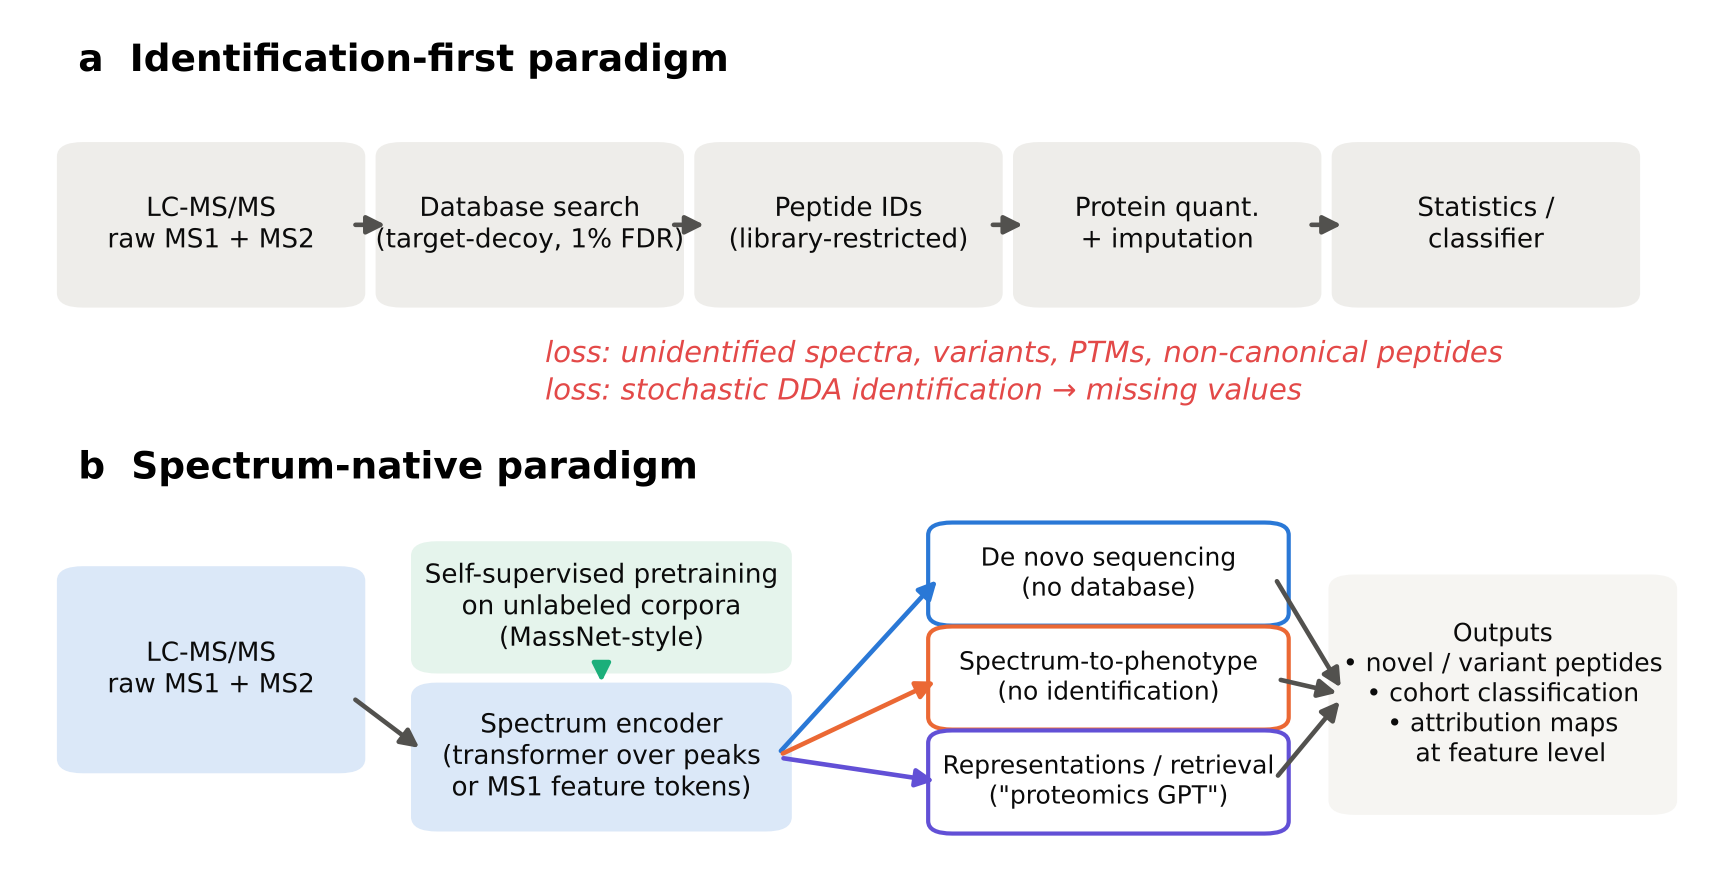
\includegraphics[width=\textwidth]{figures/fig1_paradigm.png}
\caption{\textbf{From identification-first to spectrum-native proteomics.} (a) The classical workflow loses unidentified spectra, variants, PTMs and non-canonical peptides at the search step, and creates missing values through stochastic DDA identification. (b) Spectrum-native models share an encoder that may be pretrained on unlabeled corpora and support database-free sequencing, identification-free phenotype prediction and representation learning.}\label{fig:1}
\end{figure}

\begin{figure}[htbp]
\centering
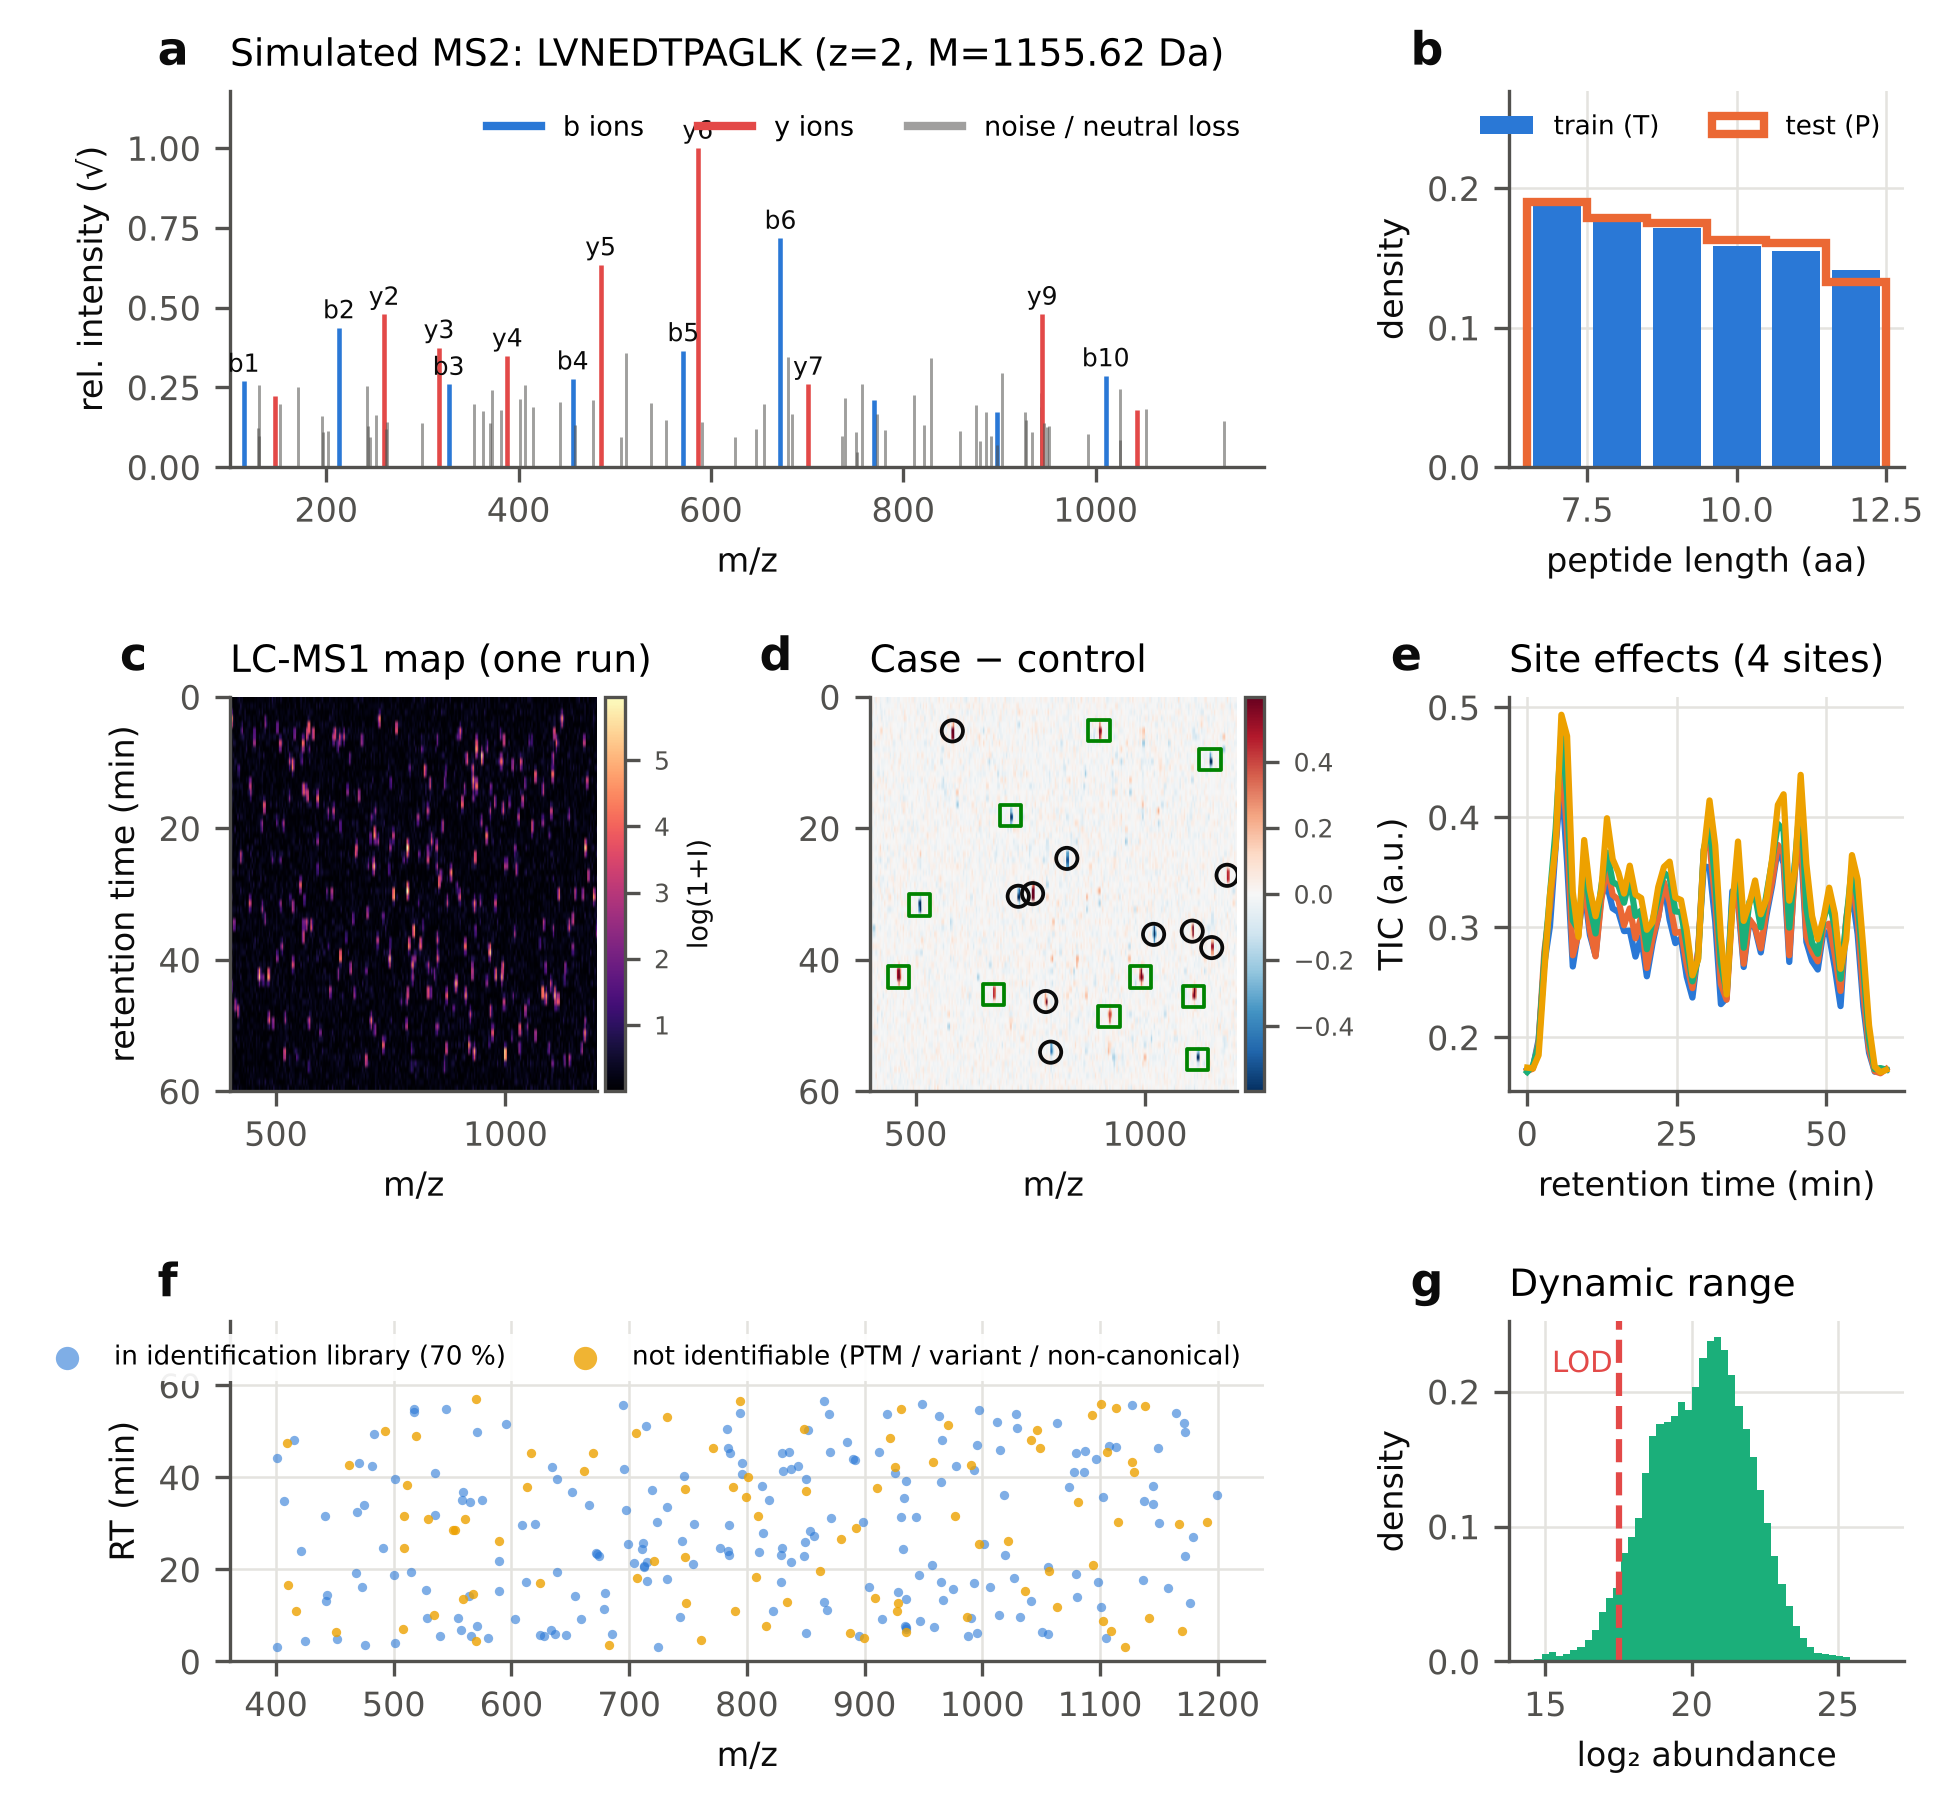
\includegraphics[width=\textwidth]{figures/fig2_virtual_instrument.png}
\caption{\textbf{The virtual instrument.} (a) Simulated MS2 spectrum of LVNEDTPAGLK with annotated b (blue) and y (red) ions; grey, noise and neutral-loss peaks. (b) Peptide-length distributions of training (proteome T) and test (proteome P) spectra. (c) Rendered LC-MS1 map of one run (64 RT × 256 m/z bins). (d) Mean case − control difference map; circles, library biomarkers; squares, unidentifiable biomarkers. (e) Total-ion chromatograms of the four acquisition sites. (f) MS1 feature landscape coloured by identifiability. (g) Abundance distribution and limit of detection (LOD).}\label{fig:2}
\end{figure}

\begin{table}[htbp]
\footnotesize
\caption{Benchmark corpora generated by the virtual instrument.}\label{tab:1}
\setlength{\tabcolsep}{4pt}
\begin{tabularx}{\textwidth}{@{}>{\raggedright\arraybackslash\hsize=0.507\hsize}X>{\raggedright\arraybackslash\hsize=0.946\hsize}X>{\raggedright\arraybackslash\hsize=1.520\hsize}X>{\raggedright\arraybackslash\hsize=0.507\hsize}X>{\raggedright\arraybackslash\hsize=1.520\hsize}X@{}}
\toprule
Corpus / set & Source & Spectra & Unique peptides & Condition \\
\midrule
Training & proteome T (3,000 proteins) & 250,000 & 73,126 & \emph{p}\textsubscript{obs} ∼ U(0.55, 0.95), λ ∼ U(10, 100) \\
Validation & proteome T & 2,000 & – & \emph{p}\textsubscript{obs} = 0.80, λ = 40 \\
inDB & proteome P (in database) & 3,000 & 3,000 & \emph{p}\textsubscript{obs} = 0.80, λ = 40 \\
SAAV & P + single AA variant & 1,500 & 1,500 & \emph{p}\textsubscript{obs} = 0.80, λ = 40 \\
novel & proteome N (not in DB) & 1,500 & 1,500 & \emph{p}\textsubscript{obs} = 0.80, λ = 40 \\
Robustness ×8 & proteome P & 8 × 1,000 & – & \emph{p}\textsubscript{obs} ∈ \{0.95, 0.80, 0.65, 0.50\}; λ ∈ \{10,40,100,200\} \\
Search database & proteome P targets (+Met-ox) & – & 45,779 & + equal number of reversed decoys \\
MS1 cohorts & 300 features, 4 sites & 800 unlabeled + 384 labelled + 500 test runs / seed & – & 20 biomarkers, absolute log₂FC 0.26–0.44 \\
\botrule
\end{tabularx}
\end{table}

\begin{table}[htbp]
\small
\caption{Model and training configurations.}\label{tab:2}
\setlength{\tabcolsep}{4pt}
\begin{tabularx}{\textwidth}{@{}>{\raggedright\arraybackslash\hsize=0.404\hsize}X>{\raggedright\arraybackslash\hsize=1.298\hsize}X>{\raggedright\arraybackslash\hsize=1.298\hsize}X@{}}
\toprule
Item & SpecNovo & FeatureFormer \\
\midrule
Input & ≤ 80 peaks (m/z, √I) + precursor (M, z) & 300 aligned MS1 features (value or missing) \\
Embedding & sinusoidal m/z (λ 10⁻³–10⁴ Da) + complementary m/z + intensity & feature ID + 0.1·sin(m/z, RT) + value × w\_j (FT-style) \\
Encoder & 3 × pre-norm transformer, d = 128, 4 heads, FF 512 & 2 × pre-norm transformer, d = 64, 4 heads, FF 128 \\
Decoder / head & 3-layer autoregressive decoder + prefix/residual mass + ion-evidence MLP (8→32→1) & [CLS] logit + zero-initialised additive token evidence \\
Parameters & 1.44 M & 0.14 M \\
Objective & cross-entropy, label smoothing 0.05 & SSL: masked-intensity MSE (30 \%); fine-tune: cross-entropy, smoothing 0.1 \\
Optimiser & AdamW, lr 5 × 10⁻⁴ (3 × 10⁻⁴ for evidence stage), cosine, batch 128 & AdamW, one-cycle, lr 10⁻³ (head) / 2 × 10⁻⁴ (body), batch 32, 150 steps \\
Inference & beam K = 5, precursor-mass constraint 0.05 Da & single forward pass \\
Hardware & 3 CPU threads; final model ≈ 1.45 h wall-clock (mass-aware + evidence stages) & 1 CPU thread per seed \\
\botrule
\end{tabularx}
\end{table}

\begin{figure}[htbp]
\centering
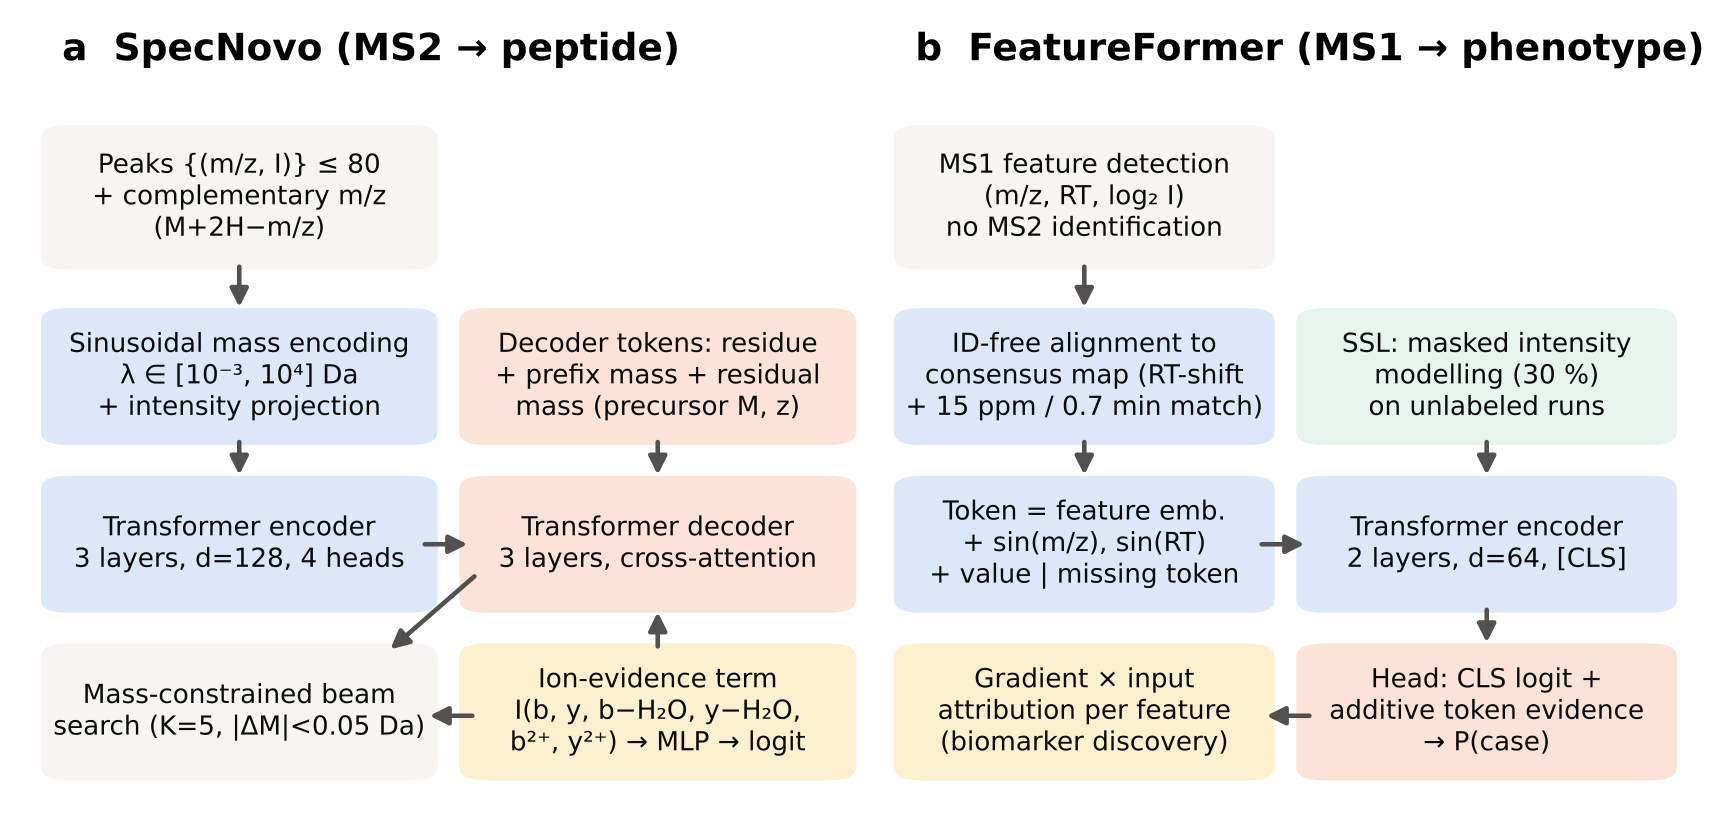
\includegraphics[width=\textwidth]{figures/fig3_architecture.png}
\caption{\textbf{Model architectures.} (a) SpecNovo encodes peaks and their complementary masses, decodes residues conditioned on prefix and residual mass, and adds a differentiable ion-evidence logit; decoding is mass-constrained. (b) FeatureFormer tokenises identification-free MS1 features, is pretrained by masked-intensity modelling on unlabeled runs and fine-tuned for phenotype; gradient × input yields feature-level attributions.}\label{fig:3}
\end{figure}

\subsection{Database-free sequencing recovers peptides that database search cannot}

On canonical peptides, target--decoy database search was essentially perfect: recall 0.999 at 1 \% FDR, with 0.03 \% false identifications (Table\textasciitilde{}\ref{tab:3}, Fig.\textasciitilde{}\ref{fig:4}c). This is the regime for which identification-first proteomics was designed. Introducing a single amino-acid variant, or drawing peptides from a proteome absent from the database, reduced database-search recall to 0.000 (Table\textasciitilde{}\ref{tab:3}). Target--decoy competition correctly rejected the near-miss target matches, so no false identifications passed 1 \% FDR; but every variant and novel peptide was lost.

Both de novo methods were, as expected, insensitive to database membership. SpecNovo recall was 0.416, 0.389 and 0.387, and spectrum-graph recall 0.475, 0.475 and 0.468, on the canonical, SAAV and novel sets respectively.

At full coverage the classical spectrum-graph algorithm had higher peptide recall and amino-acid precision (0.834 vs 0.687 on inDB). SpecNovo, however, produced better-ranked confidence scores, with precision--coverage AUC of 0.663 vs 0.630 (Fig.\textasciitilde{}\ref{fig:4}b). Its precision was higher whenever predictions were filtered by confidence:

\begin{center}\small
\setlength{\tabcolsep}{4pt}
\begin{tabularx}{0.7\textwidth}{@{}>{\raggedright\arraybackslash\hsize=0.789\hsize}X>{\raggedright\arraybackslash\hsize=0.947\hsize}X>{\raggedright\arraybackslash\hsize=1.263\hsize}X@{}}
\toprule
Coverage (inDB) & SpecNovo precision & Spectrum-graph precision \\
\midrule
10 \% & 0.874 & 0.801 \\
25 \% & 0.787 & 0.716 \\
50 \% & 0.660 & 0.612 \\
\botrule
\end{tabularx}
\end{center}

The same held for SAAV spectra, where precision at 10 \% coverage was 0.905 vs 0.743. In practice, this is the regime that matters for database-free discovery, where only high-confidence de novo calls are followed up.

\begin{table}[htbp]
\footnotesize
\caption{Database-dependent and database-free peptide identification.}\label{tab:3}
\setlength{\tabcolsep}{3pt}
\begin{tabularx}{\textwidth}{@{}>{\raggedright\arraybackslash\hsize=0.667\hsize}X>{\raggedright\arraybackslash\hsize=1.333\hsize}X>{\raggedright\arraybackslash\hsize=1.000\hsize}X>{\raggedright\arraybackslash\hsize=0.750\hsize}X>{\raggedright\arraybackslash\hsize=1.167\hsize}X>{\raggedright\arraybackslash\hsize=0.500\hsize}X>{\raggedright\arraybackslash\hsize=1.583\hsize}X@{}}
\toprule
Test set & Method & AA precision & AA recall & Peptide recall & PR-AUC & False IDs (1 \% FDR) \\
\midrule
inDB & DB-search & – & – & 0.999 & – & 0.000 \\
inDB & SpectrumGraph-DP & 0.834 & 0.876 & 0.475 & 0.630 & – \\
inDB & SpecNovo & 0.687 & 0.698 & 0.416 & 0.663 & – \\
SAAV & DB-search & – & – & 0.000 & – & 0.000 \\
SAAV & SpectrumGraph-DP & 0.835 & 0.877 & 0.475 & 0.615 & – \\
SAAV & SpecNovo & 0.670 & 0.684 & 0.389 & 0.646 & – \\
novel & DB-search & – & – & 0.000 & – & 0.000 \\
novel & SpectrumGraph-DP & 0.832 & 0.876 & 0.468 & 0.622 & – \\
novel & SpecNovo & 0.670 & 0.684 & 0.387 & 0.634 & – \\
\botrule
\end{tabularx}
\end{table}

\begin{figure}[htbp]
\centering
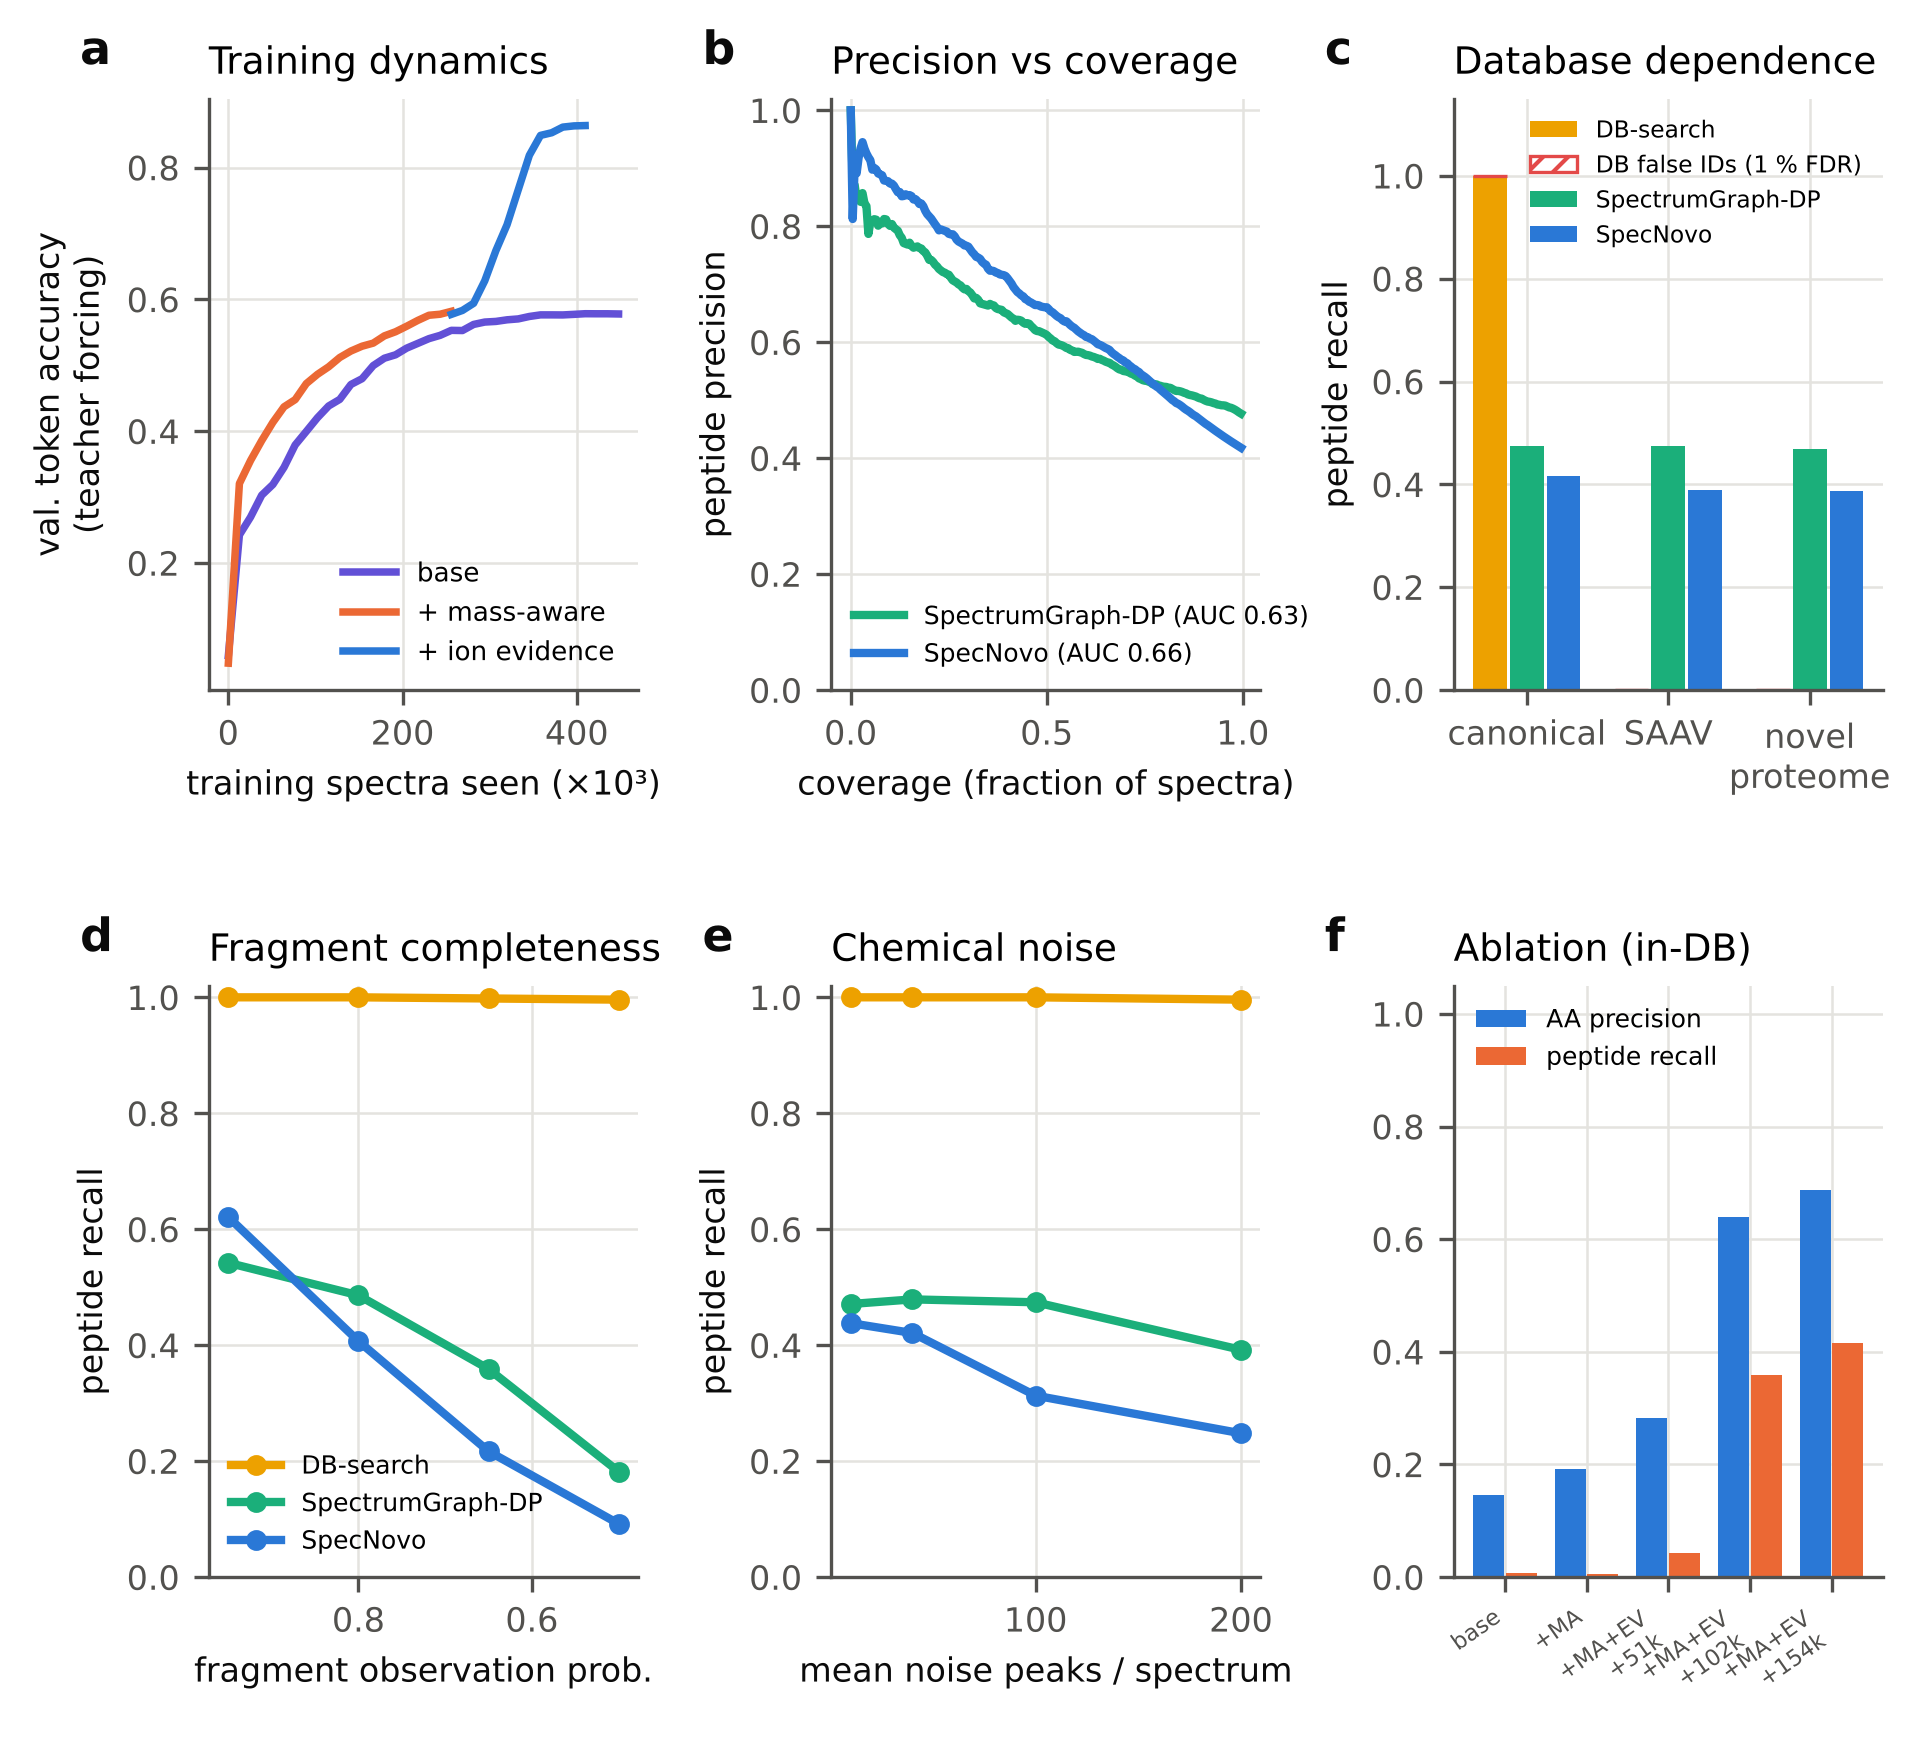
\includegraphics[width=\textwidth]{figures/fig4_denovo.png}
\caption{\textbf{De novo sequencing benchmark.} (a) Validation token accuracy (teacher forcing) as a function of training spectra for the base transformer, the mass-aware variant and the ion-evidence variant (initialised from the mass-aware checkpoint). (b) Peptide precision–coverage curves on inDB. (c) Peptide recall of database search, spectrum-graph DP and SpecNovo on canonical, SAAV and novel-proteome spectra; hatched, database false identifications at 1 \% FDR. (d, e) Peptide recall versus fragment observation probability and chemical-noise peaks. (f) Ablation: amino-acid precision and peptide recall on inDB; MA, mass-aware; EV, ion evidence; +Nk, additional training spectra.}\label{fig:4}
\end{figure}

\subsection{Inductive biases, not capacity, determine data efficiency}

The ablation (Table\textasciitilde{}\ref{tab:5}, Fig.\textasciitilde{}\ref{fig:4}a,f) is the most instructive result of this study. A standard Casanovo-style encoder--decoder reached a teacher-forced validation token accuracy of 0.578 after 448k training spectra. Under mass-constrained beam search, however, it achieved only 0.8 \% peptide recall and 0.146 amino-acid precision. Inspection of greedy decodes showed that the model had learned the sequence prior (C-terminal K/R, residue frequencies) but very little of the spectrum: the decodes were plausible tryptic peptides that did not explain the observed peaks.

Complementary-ion encoding and prefix/residual-mass conditioning accelerated early learning (token accuracy 0.386 vs 0.303 at 38k spectra) but saturated at the same level (0.582). Adding the differentiable ion-evidence term broke this plateau within 1,200 further optimisation steps. Token accuracy rose to 0.674, 0.849 and 0.864 after 51k, 102k and 154k additional spectra, and peptide recall rose to 4.3 \%, 35.9 \% and 41.6 \%. The total budget (410k spectra, ≈ 1.45 h of wall-clock time on three CPU threads) is two orders of magnitude below that used to train published de novo transformers (e.g., 30 M spectra for Casanovo \cite{yilmaz2024}). The ablation therefore quantifies how much a physics-informed prior substitutes for data. It also explains why repository-scale corpora are a precondition for purely data-driven ``proteomics GPTs''.

\begin{table}[htbp]
\footnotesize
\caption{Ablation of SpecNovo inductive biases on the inDB test set (beam K = 5).}\label{tab:5}
\setlength{\tabcolsep}{3pt}
\begin{tabularx}{\textwidth}{@{}>{\raggedright\arraybackslash\hsize=2.508\hsize}X>{\raggedright\arraybackslash\hsize=0.933\hsize}X>{\raggedright\arraybackslash\hsize=1.167\hsize}X>{\raggedright\arraybackslash\hsize=0.700\hsize}X>{\raggedright\arraybackslash\hsize=0.525\hsize}X>{\raggedright\arraybackslash\hsize=0.817\hsize}X>{\raggedright\arraybackslash\hsize=0.350\hsize}X@{}}
\toprule
Variant & Training spectra & Val. token acc. (TF) & AA precision & AA recall & Peptide recall & PR-AUC \\
\midrule
Base transformer & 448k & 0.578 & 0.146 & 0.216 & 0.008 & 0.036 \\
+ complementary ions \& prefix-mass decoding & 256k & 0.582 & 0.192 & 0.214 & 0.005 & 0.021 \\
+ ion-evidence term (+400 steps) & 307k & 0.674 & 0.282 & 0.305 & 0.043 & 0.123 \\
+ ion-evidence term (+800 steps) & 358k & 0.849 & 0.639 & 0.656 & 0.359 & 0.598 \\
+ ion-evidence term (+1,200 steps, final) & 410k & 0.864 & 0.687 & 0.698 & 0.416 & 0.663 \\
\botrule
\end{tabularx}
\end{table}

\subsection{Robustness: where classical algorithms still win}

Fragment completeness was the dominant factor (Table\textasciitilde{}\ref{tab:4}, Fig.\textasciitilde{}\ref{fig:4}d). With nearly complete ladders (\emph{p}\textsubscript{obs} = 0.95), SpecNovo outperformed the spectrum graph: peptide recall 0.621 vs 0.542, PR-AUC 0.840 vs 0.693. Below \emph{p}\textsubscript{obs} ≈ 0.9 the ranking reversed, and at \emph{p}\textsubscript{obs} = 0.5 SpecNovo recalled 9.2 \% of peptides against 18.2 \% for the spectrum graph. SpecNovo was also more sensitive to chemical noise (Fig.\textasciitilde{}\ref{fig:4}e). From λ = 10 to 200 noise peaks its recall fell from 0.438 to 0.248, while the spectrum graph fell only from 0.471 to 0.392.

Database search was robust to both perturbations (≥ 0.996), confirming that the hard part of de novo sequencing is the missing information, not the spectrum quality per se. These results mark the current limits of small spectrum-native models. More training data that covers sparse and noisy spectra, or hybrid models that combine learned scoring with exhaustive graph search, are the obvious next steps.

\begin{table}[htbp]
\footnotesize
\caption{Robustness to fragment completeness and chemical noise (1,000 spectra per condition).}\label{tab:4}
\setlength{\tabcolsep}{3pt}
\begin{tabularx}{\textwidth}{@{}>{\raggedright\arraybackslash\hsize=0.882\hsize}X>{\raggedright\arraybackslash\hsize=1.235\hsize}X>{\raggedright\arraybackslash\hsize=1.647\hsize}X>{\raggedright\arraybackslash\hsize=1.176\hsize}X>{\raggedright\arraybackslash\hsize=0.647\hsize}X>{\raggedright\arraybackslash\hsize=1.000\hsize}X>{\raggedright\arraybackslash\hsize=0.529\hsize}X>{\raggedright\arraybackslash\hsize=0.882\hsize}X@{}}
\toprule
Condition & DB-search pep. recall & SpectrumGraph-DP pep. recall & SpecNovo pep. recall & DP AA prec. & SpecNovo AA prec. & DP PR-AUC & SpecNovo PR-AUC \\
\midrule
\emph{p}\textsubscript{obs} = 0.95 & 1.000 & 0.542 & 0.621 & 0.865 & 0.808 & 0.693 & 0.840 \\
\emph{p}\textsubscript{obs} = 0.80 & 1.000 & 0.486 & 0.407 & 0.841 & 0.679 & 0.623 & 0.640 \\
\emph{p}\textsubscript{obs} = 0.65 & 0.998 & 0.359 & 0.217 & 0.776 & 0.533 & 0.504 & 0.440 \\
\emph{p}\textsubscript{obs} = 0.50 & 0.996 & 0.182 & 0.092 & 0.655 & 0.393 & 0.312 & 0.216 \\
λ = 10 & 1.000 & 0.471 & 0.438 & 0.844 & 0.707 & 0.619 & 0.669 \\
λ = 40 & 1.000 & 0.479 & 0.421 & 0.836 & 0.673 & 0.641 & 0.686 \\
λ = 100 & 1.000 & 0.474 & 0.313 & 0.833 & 0.625 & 0.620 & 0.535 \\
λ = 200 & 0.996 & 0.392 & 0.248 & 0.784 & 0.526 & 0.540 & 0.495 \\
\botrule
\end{tabularx}
\end{table}

\subsection{Learned representations and peak-level attribution}

We tested whether the SpecNovo encoder learns peptide identity without being trained to do so. We generated 12 independent noisy replicate spectra for each of 40 test peptides (\emph{p}\textsubscript{obs} = 0.75, λ = 60) and compared mean-pooled encoder embeddings with 0.5 Da binned spectra (Fig.\textasciitilde{}\ref{fig:5}a--c, Table\textasciitilde{}\ref{tab:8}).

The encoder embedding grouped replicates more compactly: cosine silhouette 0.273 vs 0.222. Its top-1 replicate retrieval (0.908) was slightly below that of binned spectra (0.996). In simulation, replicate spectra share exact fragment m/z values, which favours binned matching; on real data with calibration drift, learned embeddings such as GLEAMS \cite{bittremieux2022} are expected to have the advantage.

Gradient × input attribution showed that SpecNovo bases its predictions on genuine fragment ions (Fig.\textasciitilde{}\ref{fig:5}d,e). Annotated b/y-family ions carried 42.2 \% of the total intensity but received 80.0 \% of the attribution mass, and attribution exceeded the intensity share in 299 of 300 spectra. The model therefore actively down-weights noise peaks, an interpretable behaviour that classical intensity-weighted scores do not provide.

\begin{figure}[htbp]
\centering
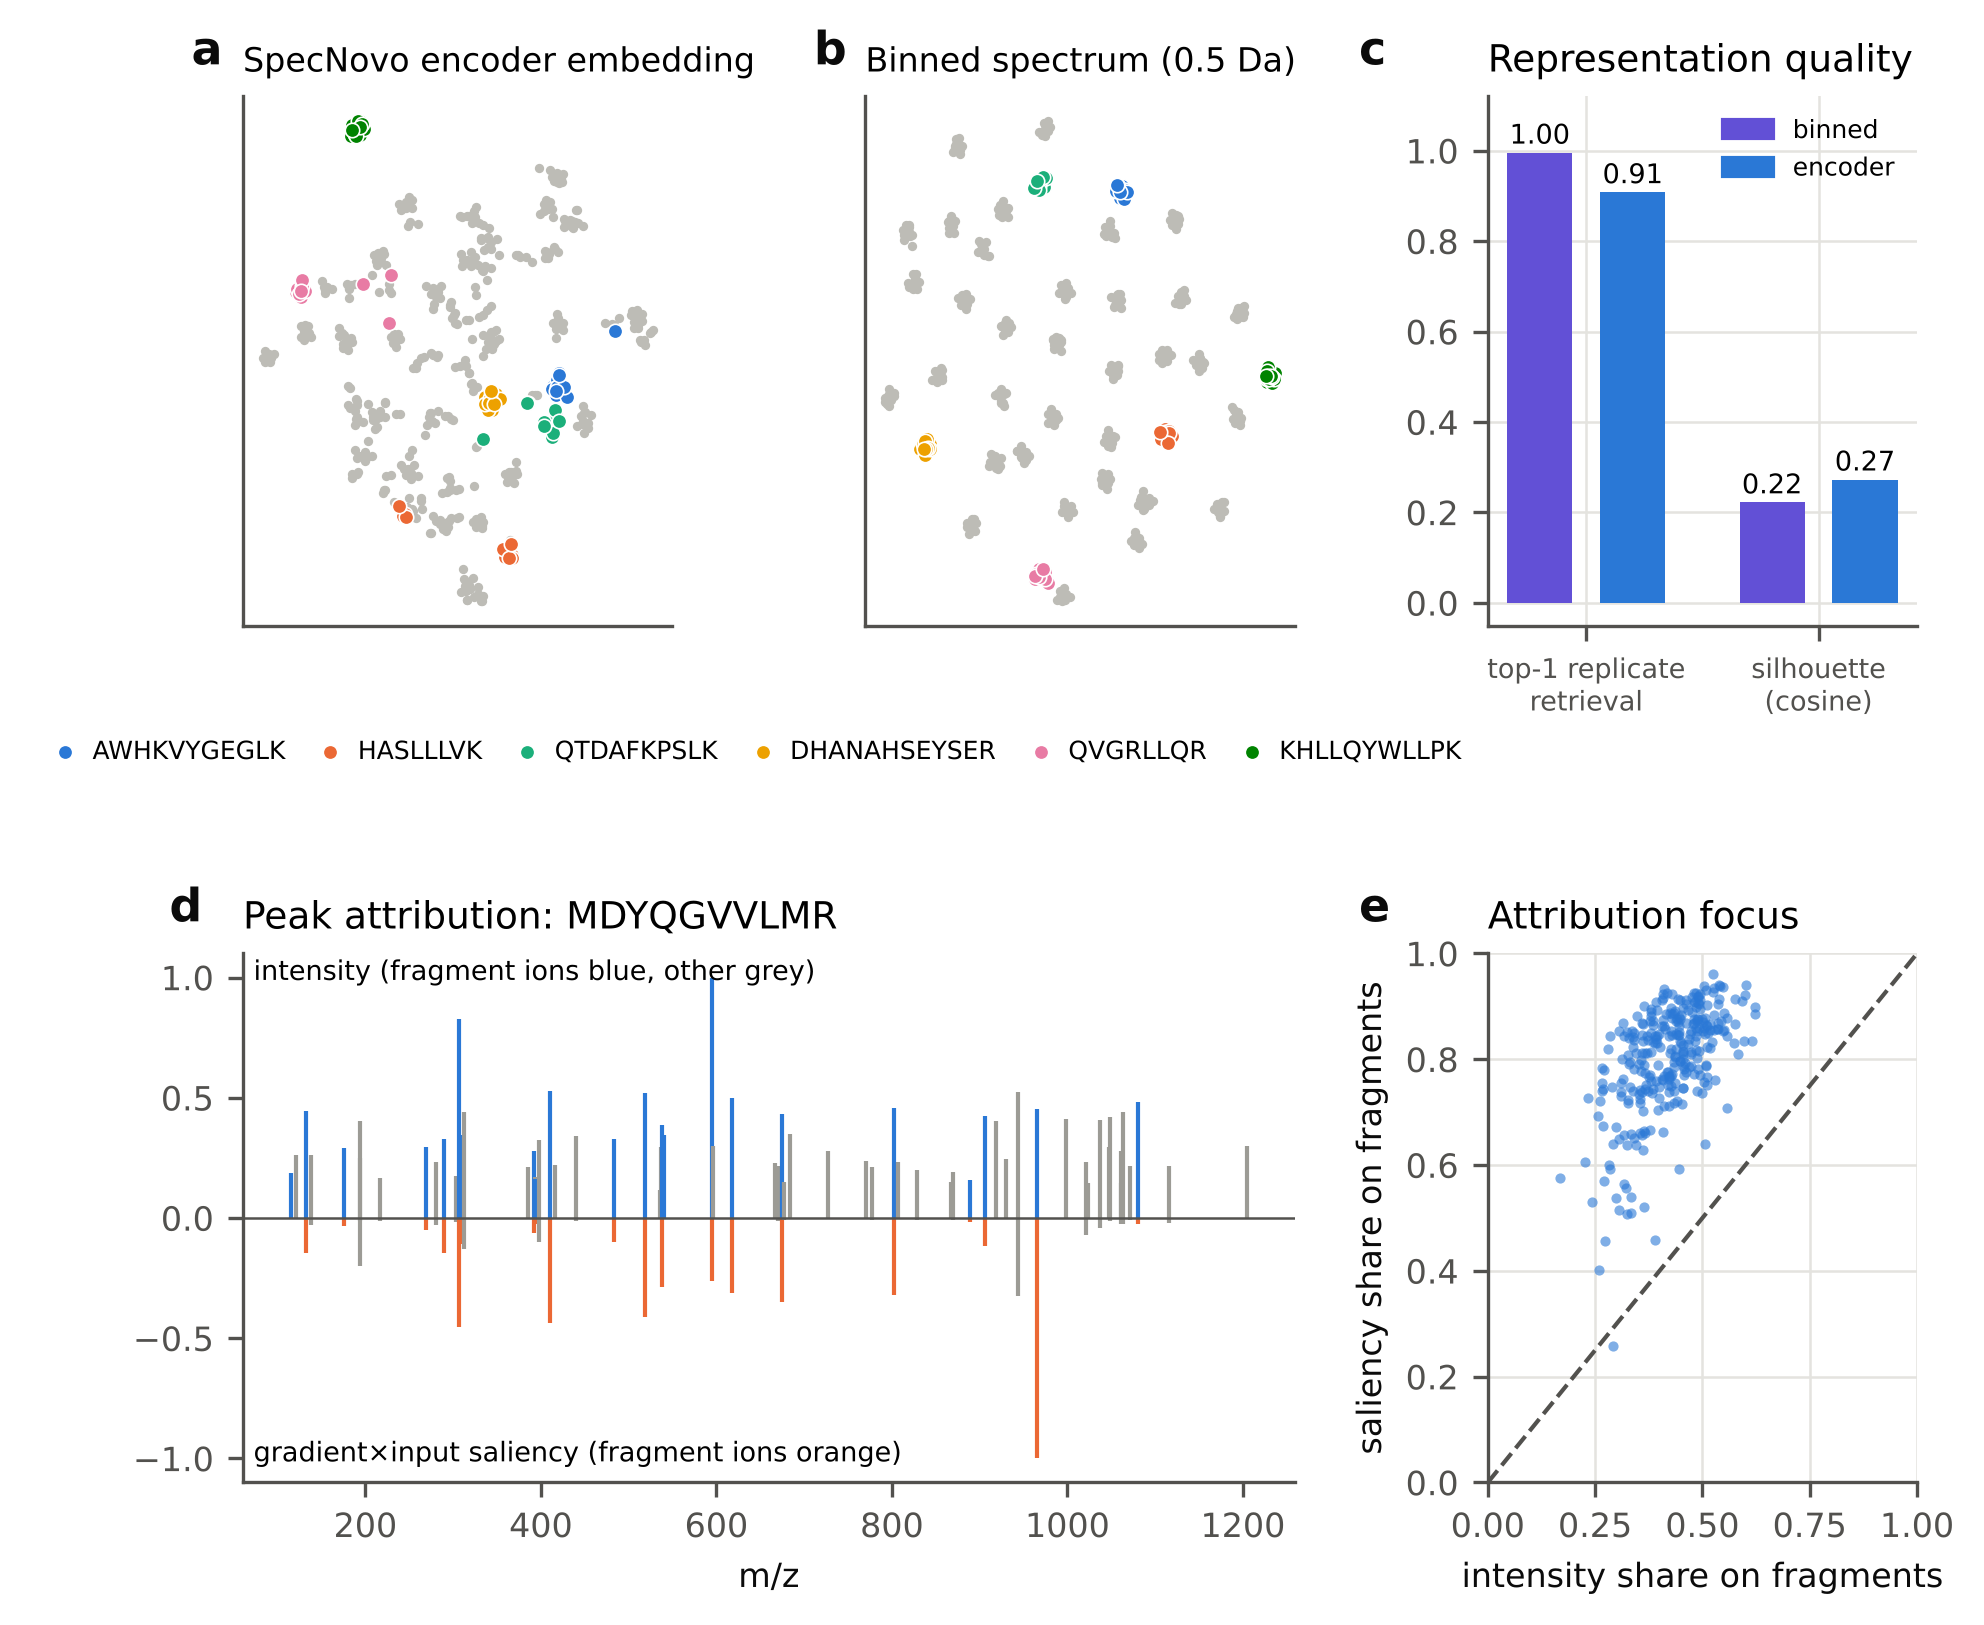
\includegraphics[width=\textwidth]{figures/fig5_representation.png}
\caption{\textbf{Representations and interpretability of SpecNovo.} (a, b) t-SNE of 480 replicate spectra (40 peptides × 12) using encoder embeddings (a) or binned spectra (b); six peptides highlighted. (c) Top-1 replicate retrieval and cosine silhouette. (d) Example spectrum: intensity (top; fragment ions blue) and gradient × input saliency (bottom; fragment ions orange). (e) Saliency share versus intensity share on annotated fragment ions for 300 inDB spectra; dashed line, identity.}\label{fig:5}
\end{figure}

\begin{table}[htbp]
\small
\caption{Representation quality, interpretability and compute.}\label{tab:8}
\setlength{\tabcolsep}{4pt}
\begin{tabularx}{\textwidth}{@{}>{\raggedright\arraybackslash\hsize=1.406\hsize}X>{\raggedright\arraybackslash\hsize=1.406\hsize}X>{\raggedright\arraybackslash\hsize=0.188\hsize}X@{}}
\toprule
Analysis & Metric & Value \\
\midrule
Replicate retrieval (40 peptides × 12 spectra) & top-1 accuracy, encoder embedding & 0.908 \\
 & top-1 accuracy, binned spectrum (0.5 Da) & 0.996 \\
 & silhouette (cosine), encoder & 0.273 \\
 & silhouette (cosine), binned & 0.222 \\
Peak attribution (300 inDB spectra) & mean saliency share on annotated fragment ions & 0.800 \\
 & mean intensity share on annotated fragment ions & 0.422 \\
Inference cost & CPU seconds per 1,000 spectra (beam K=5, 2 threads) & 155 \\
Feature attribution (seed 0, n = 384) & AUROC of abs(grad × input) for true biomarkers & 0.622 \\
 & AUROC of Welch t-test −log10 p (ID-free matrix) & 1.000 \\
\botrule
\end{tabularx}
\end{table}

\subsection{Spectrum-to-phenotype: removing the identification bottleneck}

The same theme dominated the MS1 experiments, at the cohort level (Table\textasciitilde{}\ref{tab:6}, Fig.\textasciitilde{}\ref{fig:6}). With half of the biomarkers unidentifiable, the identification-first pipeline reached AUROC 0.558 with 24 labelled runs and 0.672 with 384 (Fig.\textasciitilde{}\ref{fig:6}a). Two losses compound here: unidentified biomarkers, and 25 \% missing values from stochastic DDA identification, which minimum-value imputation turns into noise.

Match-between-runs (MBR) recovered the missing-value loss but not the unidentified biomarkers (0.932 at n = 192). The identification-free linear model, which uses all aligned features, was best at every label budget: 0.820 at n = 24, 0.975 at n = 192 and 0.981 at n = 384. The ProFormer-style FeatureFormer improved substantially on identification-first statistics (0.767 vs 0.648 at n = 192; 0.802 vs 0.672 at n = 384). At these sample sizes it did not reach the identification-free linear model, because the simulated phenotype signal is additive and linear models are near-optimal for it.

Self-supervised masked-intensity pretraining on 800 unlabeled runs did not improve in-distribution accuracy (0.714 vs 0.767 at n = 192). It did improve transfer to an unseen acquisition site: leave-one-site-out AUROC rose from 0.651 ± 0.087 to 0.728 ± 0.054, with lower variance (Fig.\textasciitilde{}\ref{fig:6}b). Identification-free features also transferred best overall (0.986 ± 0.012), because ID-free RT-shift alignment absorbs site-specific chromatographic drift.

\begin{table}[htbp]
\footnotesize
\caption{Spectrum-to-phenotype AUROC (mean ± s.d. over three seeds; 500 test runs; 50 \% of biomarkers unidentifiable).}\label{tab:6}
\setlength{\tabcolsep}{3pt}
\begin{tabularx}{\textwidth}{@{}>{\raggedright\arraybackslash\hsize=1.190\hsize}X>{\raggedright\arraybackslash\hsize=0.910\hsize}X>{\raggedright\arraybackslash\hsize=0.910\hsize}X>{\raggedright\arraybackslash\hsize=0.910\hsize}X>{\raggedright\arraybackslash\hsize=0.910\hsize}X>{\raggedright\arraybackslash\hsize=0.910\hsize}X>{\raggedright\arraybackslash\hsize=1.260\hsize}X@{}}
\toprule
Method & n = 24 & n = 48 & n = 96 & n = 192 & n = 384 & LOSO (unseen site) \\
\midrule
ID-first-LR & 0.558 ± 0.050 & 0.587 ± 0.034 & 0.606 ± 0.007 & 0.648 ± 0.013 & 0.672 ± 0.040 & 0.627 ± 0.034 \\
ID-first+MBR-LR & 0.660 ± 0.070 & 0.818 ± 0.031 & 0.864 ± 0.005 & 0.932 ± 0.020 & 0.945 ± 0.021 & 0.942 ± 0.019 \\
ID-free-LR & 0.820 ± 0.046 & 0.903 ± 0.003 & 0.942 ± 0.017 & 0.975 ± 0.015 & 0.981 ± 0.015 & 0.986 ± 0.012 \\
FeatureFormer & 0.661 ± 0.041 & 0.695 ± 0.023 & 0.693 ± 0.044 & 0.767 ± 0.037 & 0.802 ± 0.018 & 0.651 ± 0.087 \\
FeatureFormer+SSL & 0.593 ± 0.026 & 0.652 ± 0.042 & 0.674 ± 0.020 & 0.714 ± 0.015 & 0.737 ± 0.025 & 0.728 ± 0.054 \\
\botrule
\end{tabularx}
\end{table}

\begin{figure}[htbp]
\centering
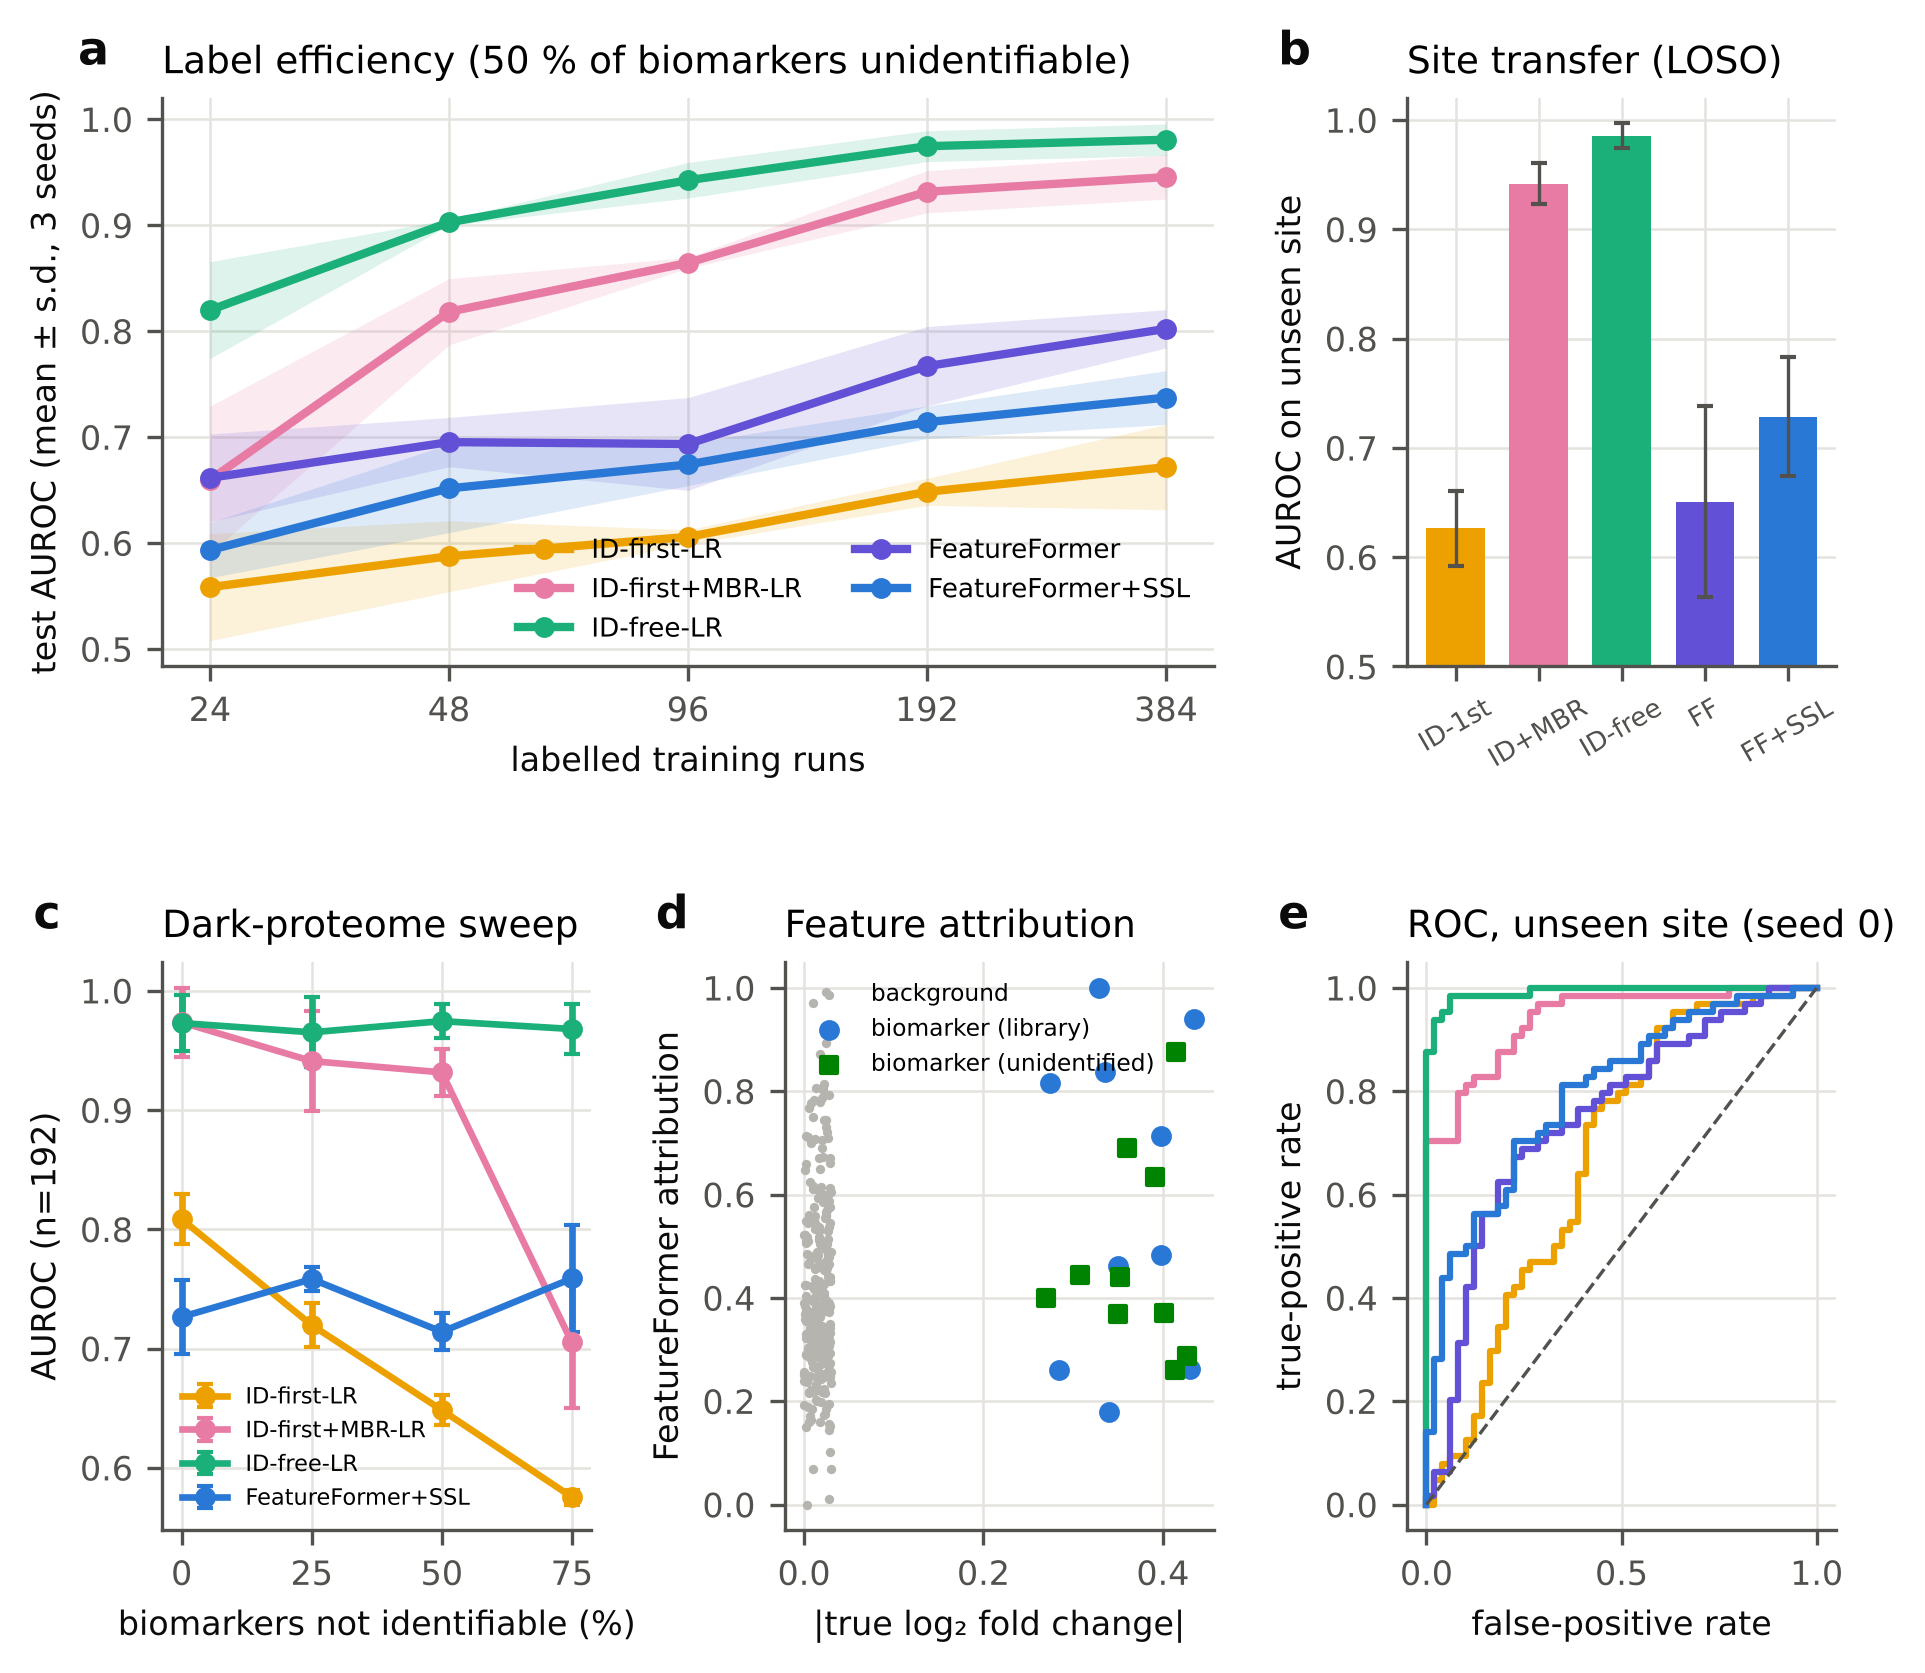
\includegraphics[width=\textwidth]{figures/fig6_phenotype.png}
\caption{\textbf{Spectrum-to-phenotype benchmark.} (a) Test AUROC versus number of labelled runs (mean ± s.d., three seeds; 50 \% of biomarkers unidentifiable). (b) Leave-one-site-out AUROC on an unseen acquisition site. (c) AUROC (n = 192) versus fraction of biomarkers not identifiable by MS2 search. (d) FeatureFormer gradient × input attribution versus true effect size; library (circles) and unidentifiable (squares) biomarkers. (e) ROC curves on the unseen site (seed 0; colours as in a).}\label{fig:6}
\end{figure}

\subsection{The dark-proteome sweep quantifies information loss}

Varying the fraction of unidentifiable biomarkers from 0 \% to 75 \% separated the pipelines cleanly (Table\textasciitilde{}\ref{tab:7}, Fig.\textasciitilde{}\ref{fig:6}c). Identification-free linear models were invariant to identifiability (0.973 → 0.968). Identification-first AUROC declined monotonically (0.808 → 0.575), approaching chance once three quarters of the biomarkers were dark. MBR matched identification-free performance while most biomarkers were identifiable (0.973 at 0 \%) but collapsed at 75 \% (0.705 ± 0.055). FeatureFormer+SSL was likewise invariant to identifiability (0.714--0.759), confirming that it uses unidentified signal, but it remained limited by sample size.

Feature attribution recovered true biomarkers above chance (AUROC 0.622), including unidentifiable ones (Fig.\textasciitilde{}\ref{fig:6}d). However, a Welch t-test on identification-free features ranked all 20 biomarkers above all background features (AUROC 1.000). For biomarker \emph{discovery} in additive settings, simple statistics on identification-free features therefore remain the reference against which deep attribution must be judged.

\begin{table}[htbp]
\footnotesize
\caption{AUROC (n = 192) as a function of the fraction of biomarkers that are not identifiable by MS2 database search.}\label{tab:7}
\setlength{\tabcolsep}{4pt}
\begin{tabularx}{\textwidth}{@{}>{\raggedright\arraybackslash\hsize=1.232\hsize}X>{\raggedright\arraybackslash\hsize=0.942\hsize}X>{\raggedright\arraybackslash\hsize=0.942\hsize}X>{\raggedright\arraybackslash\hsize=0.942\hsize}X>{\raggedright\arraybackslash\hsize=0.942\hsize}X@{}}
\toprule
Method & 0 \% & 25 \% & 50 \% & 75 \% \\
\midrule
ID-first-LR & 0.808 ± 0.021 & 0.720 ± 0.019 & 0.648 ± 0.013 & 0.575 ± 0.006 \\
ID-first+MBR-LR & 0.973 ± 0.029 & 0.941 ± 0.042 & 0.932 ± 0.020 & 0.705 ± 0.055 \\
ID-free-LR & 0.973 ± 0.024 & 0.965 ± 0.029 & 0.975 ± 0.015 & 0.968 ± 0.021 \\
FeatureFormer+SSL & 0.727 ± 0.031 & 0.758 ± 0.010 & 0.714 ± 0.015 & 0.759 ± 0.045 \\
\botrule
\end{tabularx}
\end{table}

\subsection{Validation on real PRIDE and MassIVE-KB data}

\textbf{Real spectra are sparser and more y-dominated than the default simulator} (Table\textasciitilde{}\ref{tab:9}, Fig.\textasciitilde{}\ref{fig:7}c). On 126 MassIVE-KB HCD spectra the median b-ion observation rate was 0.29 (IQR 0.14--0.50) against 0.78 in the default simulator, while y-ion observation was 0.67 (0.50--0.86). Summed y/b intensity was 2.7 against 1.7, and b/y-family ions explained 32 \% of the total ion current against 52 \%.

The proline effect (1.98 vs 1.73) and the number of unexplained peaks (38.5 vs 41) were close to the simulator. The fragment mass error was tighter in the real data (s.d. 4.4 ppm against 8.9 ppm). PRIDE BSA ion-trap CID spectra were different again: about 145 peaks per spectrum, 59 \% of the ion current explained, y/b ratio 4.1 and fragment errors of several hundred ppm (Table\textasciitilde{}\ref{tab:9}). These measurements identify the simulator's main miscalibration as the overly symmetric b/y fragmentation.

\begin{table}[htbp]
\small
\caption{Calibration of the virtual instrument against real annotated spectra (median [IQR] per PSM).}\label{tab:9}
\setlength{\tabcolsep}{4pt}
\begin{tabularx}{\textwidth}{@{}>{\raggedright\arraybackslash\hsize=1.474\hsize}X>{\raggedright\arraybackslash\hsize=0.800\hsize}X>{\raggedright\arraybackslash\hsize=0.884\hsize}X>{\raggedright\arraybackslash\hsize=0.842\hsize}X@{}}
\toprule
Statistic & Simulator (default) & MassIVE-KB HCD (real) & PRIDE BSA CID (real) \\
\midrule
PSMs analysed & 500 & 126 & 64 \\
b-ion observation rate & 0.78 [0.67–0.88] & 0.29 [0.14–0.50] & 0.69 [0.50–0.79] \\
y-ion observation rate & 0.78 [0.67–0.88] & 0.67 [0.50–0.86] & 0.83 [0.67–0.89] \\
Summed y/b intensity & 1.66 [1.12–2.27] & 2.66 [1.59–4.78] & 4.08 [2.51–6.44] \\
Pro N-terminal cleavage enhancement & 1.73 [0.91–2.77] & 1.98 [1.25–3.69] & 2.09 [0.98–3.29] \\
Fraction of TIC explained & 0.52 [0.44–0.60] & 0.32 [0.24–0.43] & 0.59 [0.45–0.68] \\
Peaks per spectrum & 62 [55–68] & 53 [38–70] & 145 [114–192] \\
Unexplained peaks & 41 [37–45] & 38.5 [26–55] & 116.5 [90–162] \\
Fragment mass error (s.d.) & 8.9 ppm & 4.4 ppm & 323 ppm (ion trap) \\
\botrule
\end{tabularx}
\end{table}

\textbf{Identification on real PRIDE runs reproduces the identification bottleneck.} The binomial-score search separated targets from decoys (Fig.\textasciitilde{}\ref{fig:7}b) and accepted 64 PSMs (20 unique BSA peptides) at 1 \% FDR. That is 2.0 \% of the 3,135 MS2 spectra; under the conservative (\emph{d} + 1)/\emph{t} estimator, 88 PSMs passed at 5 \% FDR.

On the MS1 level, feature detection found 25,613 de-isotoped features across the six files (Table\textasciitilde{}\ref{tab:11}, Fig.\textasciitilde{}\ref{fig:7}e). Of these, 2,355 (9.2 \%) were sampled for MS2 and only 48 (0.19 \%) carried a 1 \% FDR identification. After ID-free alignment of the three samples, 1,342 consensus features were quantified in all three samples, against a single feature with complete identification-first profiles (Fig.\textasciitilde{}\ref{fig:7}f).

These numbers overstate the bottleneck in absolute terms. Our minimal search engine identifies far fewer spectra than production engines (MS-GF+, Comet, Andromeda) with rescoring, and a simple centroid-linking feature finder also counts some noise traces. The direction and the order of magnitude, however, agree with the simulation: most MS1 signal is never identified, and identification-first matrices are dominated by missing values.

\textbf{Simulation-to-real transfer of de novo sequencing} (Table\textasciitilde{}\ref{tab:10}, Fig.\textasciitilde{}\ref{fig:7}d). Applied zero-shot to 119 real MassIVE-KB HCD spectra, the simulation-trained SpecNovo recovered 7.6 \% of peptides (95 \% CI 3.4--12.6 \%) with amino-acid precision 0.261. The spectrum-graph baseline, which encodes only fragmentation physics, reached 21.8 \% (15.1--29.4 \%), a substantial sim-to-real gap for the learned model.

Fine-tuning for 800 steps on the corpus re-simulated with the measured b/y statistics doubled SpecNovo's peptide recall to 15.1 \% (9.2--21.8 \%; paired difference +7.6 points, 95 \% CI +2.5 to +13.4). Amino-acid precision rose to 0.408, and precision--coverage AUC rose to 0.352 (0.215--0.474), on a par with the spectrum graph (0.346, 0.224--0.466). Calibration did not cost simulated performance: peptide recall on the simulated inDB set rose from 0.416 to 0.525, partly from the additional training steps.

On low-resolution ion-trap CID spectra (62 PSMs ≤ 14 residues, 19 peptides), neither the zero-shot nor the HCD-calibrated SpecNovo recovered complete peptides (amino-acid precision 0.105 and 0.144). The spectrum graph, with a 0.5 Da tolerance, recovered 8.1 \%. Both de novo approaches therefore remain instrument-specific, and a learned model must be trained on, or calibrated to, the fragmentation mode and mass accuracy it will be applied to.

\begin{table}[htbp]
\footnotesize
\caption{De novo sequencing of real spectra (95 \% bootstrap CI for MassIVE-KB).}\label{tab:10}
\setlength{\tabcolsep}{3pt}
\begin{tabularx}{\textwidth}{@{}>{\raggedright\arraybackslash\hsize=1.388\hsize}X>{\raggedright\arraybackslash\hsize=1.657\hsize}X>{\raggedright\arraybackslash\hsize=0.851\hsize}X>{\raggedright\arraybackslash\hsize=0.403\hsize}X>{\raggedright\arraybackslash\hsize=0.851\hsize}X>{\raggedright\arraybackslash\hsize=0.851\hsize}X@{}}
\toprule
Data & Method & AA precision & AA recall & Peptide recall & PR-AUC \\
\midrule
MassIVE-KB HCD (n = 119) & SpectrumGraph-DP & 0.593 [0.534–0.651] & 0.511 & 0.218 [0.151–0.294] & 0.346 [0.224–0.466] \\
 & SpecNovo, zero-shot (simulation only) & 0.261 [0.211–0.313] & 0.266 & 0.076 [0.034–0.126] & 0.199 [0.086–0.313] \\
 & SpecNovo, calibrated simulation & 0.408 [0.350–0.471] & 0.405 & 0.151 [0.092–0.218] & 0.352 [0.215–0.474] \\
PRIDE BSA ion-trap CID (n = 62) & SpectrumGraph-DP (0.5 Da) & 0.292 & 0.334 & 0.081 & 0.113 \\
 & SpecNovo, zero-shot & 0.105 & 0.116 & 0.000 & 0.000 \\
 & SpecNovo, calibrated (HCD) & 0.144 & 0.154 & 0.000 & 0.000 \\
\botrule
\end{tabularx}
\end{table}

\begin{table}[htbp]
\small
\caption{The identification bottleneck on real PRIDE-derived LC-MS runs (three BSA samples × two RT fractions).}\label{tab:11}
\setlength{\tabcolsep}{4pt}
\begin{tabularx}{\textwidth}{@{}>{\raggedright\arraybackslash\hsize=1.216\hsize}X>{\raggedright\arraybackslash\hsize=0.784\hsize}X@{}}
\toprule
Quantity & Value \\
\midrule
MS2 spectra / MS1 scans & 3,135 / 1,676 \\
Target + decoy database entries & 1,725,026 \\
PSMs at 1 \% FDR (unique peptides) & 64 (20); 2.0 \% of MS2 spectra \\
De-isotoped MS1 features (six files) & 25,613 \\
Features sampled for MS2 & 2,355 (9.2 \%) \\
Features with a 1 \% FDR identification & 48 (0.19 \%) \\
Consensus features after ID-free alignment & 18,636 \\
Quantified in all three samples: ID-free / ID-first & 1,342 / 1 \\
Missing values: ID-free (all features) / ID-first (identified features) & 54.2 \% / 55.6 \% \\
Pearson r of log-intensities between samples (ID-free, complete features) & 0.44–0.64 \\
\botrule
\end{tabularx}
\end{table}

\begin{figure}[htbp]
\centering
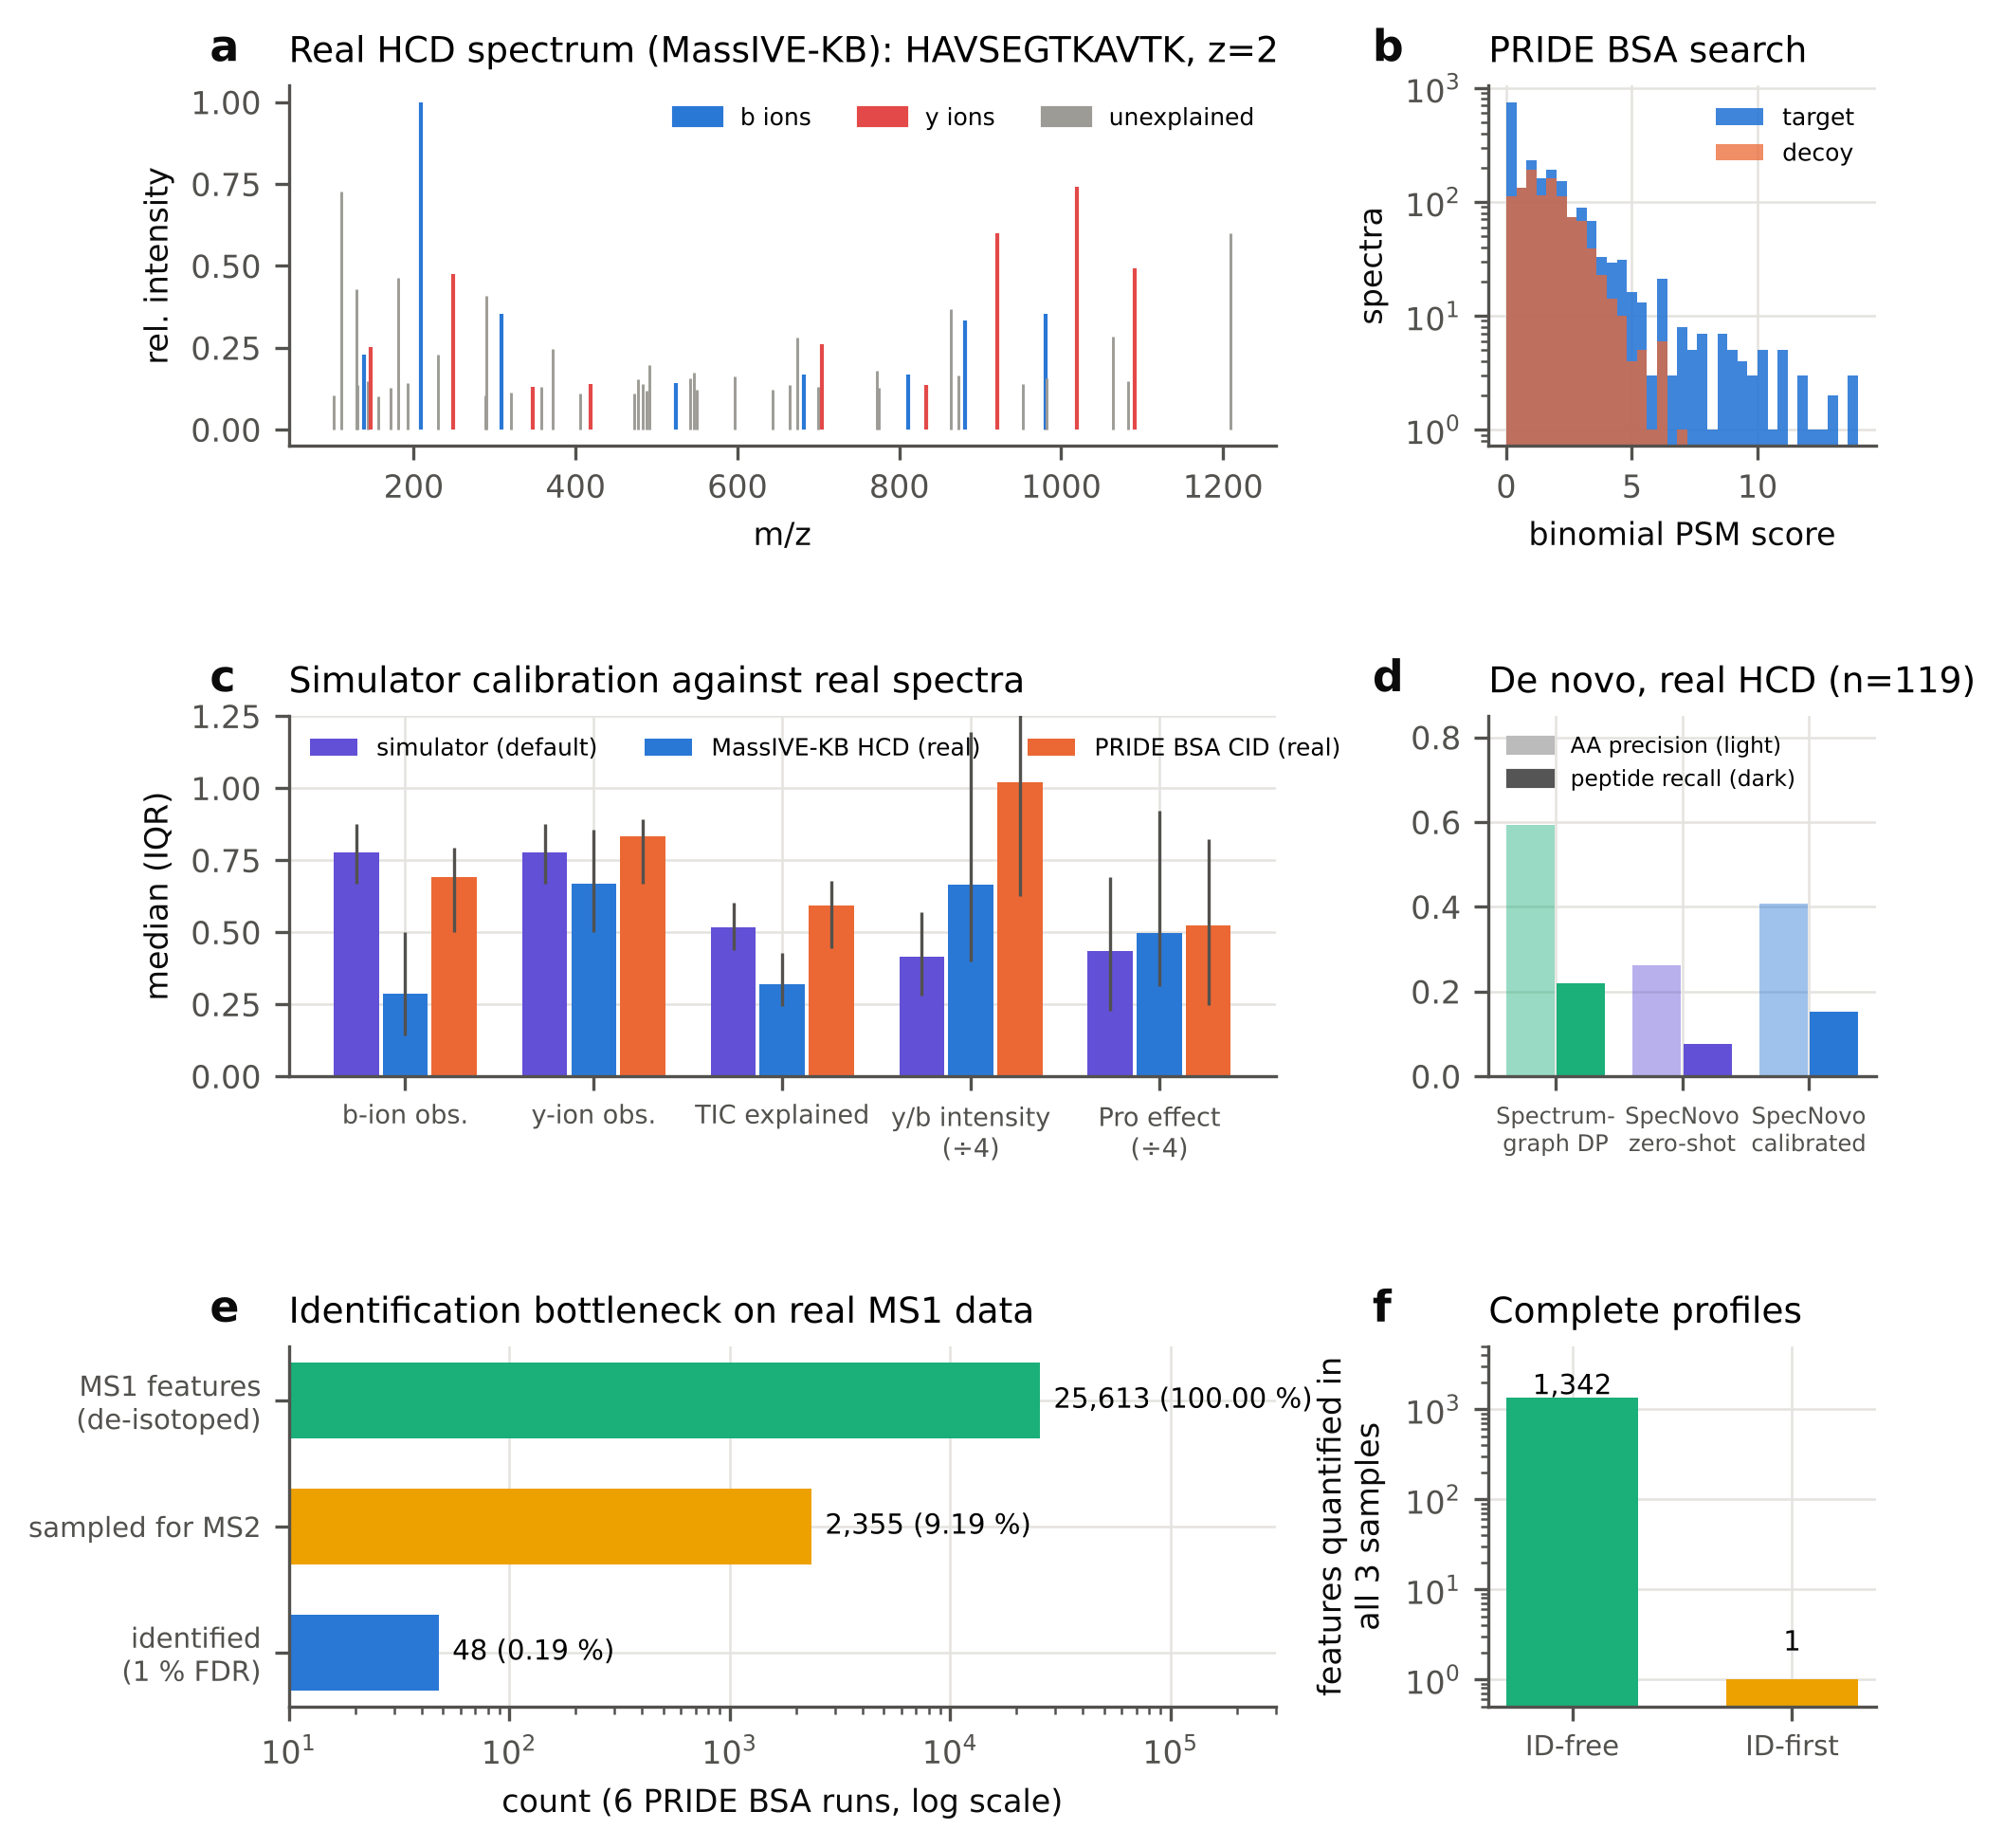
\includegraphics[width=\textwidth]{figures/fig7_real_validation.png}
\caption{\textbf{Validation on real PRIDE and MassIVE-KB data.} (a) Real annotated MassIVE-KB HCD spectrum (b ions blue, y ions red). (b) Target and decoy score distributions for the PRIDE BSA ion-trap search (log scale). (c) Fragmentation statistics of the default simulator against real HCD and CID spectra (median and IQR; ratios divided by 4 for display). (d) De novo sequencing of 119 real HCD spectra: amino-acid precision (light) and peptide recall (dark) for the spectrum-graph baseline, zero-shot SpecNovo and SpecNovo fine-tuned on calibrated simulation. (e) Identification funnel on real MS1 data: detected features, features sampled for MS2 and features with a 1 \% FDR identification. (f) Number of features quantified in all three samples with identification-free and identification-first workflows.}\label{fig:7}
\end{figure}

\section{Discussion}\label{sec:discussion}
The move from identification-first to spectrum-native proteomics is often framed as a contest between classical algorithms and deep learning. The controlled measurements here suggest a more useful framing: \textbf{identification is an information bottleneck, and the main gains come from removing that bottleneck.} The choice of model class matters less.

On the MS1 side, the bottleneck alone accounts for a 0.33 AUROC difference at n = 192 (0.648 vs 0.975), and it grows with the size of the dark proteome. This mirrors the ProFormer observation that identification-free MS1 classification is both faster and more accurate than interpretation-based workflows \cite{krull2026}. It also explains why match-between-runs is so valuable in practice \cite{cox2008}: MBR recovers the missing values, but not the biomarkers that were never identified.

On the MS2 side, database search remains unbeatable for canonical peptides but recovers nothing beyond its database. De novo sequencing provides access to variant and novel sequences at a fixed, database-independent rate, which matters for immunopeptidomics, metaproteomics, antibody sequencing and proteogenomic variant detection \cite{yilmaz2024,eloff2025}.

The second lesson concerns \textbf{data efficiency}. A generic sequence-to-sequence transformer trained on ≈ 0.45 M spectra learned a sequence language model but not spectrum interpretation, and was useless under mass-constrained decoding. A small, physics-informed ion-evidence term, analogous to the ion-location features of DeepNovo \cite{tran2017} and to pairwise mass-difference attention \cite{lapin2025}, made the same architecture competitive within a few hundred additional optimisation steps.

This result is directly relevant to the vision of proteomics GPTs trained on MassNet-style corpora. Corpus scale and inductive bias are substitutes, and at the scales available to most laboratories, inductive bias is cheaper. Conversely, the gap between our CPU-scale model and published models trained on tens of millions of spectra \cite{yilmaz2024,eloff2025} is consistent with data scaling, not architectural limits, being the main driver of state-of-the-art de novo accuracy.

Third, \textbf{self-supervised pretraining is not a free lunch at small scale.} Masked-intensity pretraining on 800 unlabeled runs did not improve in-distribution phenotype prediction, but it consistently improved cross-site transfer and reduced variance. This pattern is expected if pretraining learns site-invariant co-abundance structure rather than phenotype-specific signal. It suggests that the payoff of corpus-scale pretraining will appear first in robustness and transfer across instruments, laboratories and cohorts.

\textbf{Limitations.} The central comparisons are drawn from simulation. The real-data validation is deliberately small: 3,135 PRIDE-derived MS2 spectra and 119 MassIVE-KB spectra, obtained from public mirrors because the PRIDE archive itself could not be reached from the compute environment. It used a minimal search engine and feature finder, and it could not test phenotype prediction, which requires labelled cohorts of tens to hundreds of runs. The real data nonetheless show that the default virtual instrument overestimates b-ion completeness and that learned de novo models suffer a substantial sim-to-real gap, which calibration halves but does not close. The virtual instrument also omits several features of real data:

\begin{itemize}
\item
  fragment-intensity patterns learned from real data (e.g., Prosit or AlphaPeptDeep \cite{gessulat2019,zeng2022});
\item
  chimeric and DIA spectra;
\item
  isotope and charge-state ambiguity in precursor selection;
\item
  non-tryptic peptides;
\item
  PTMs other than Met oxidation;
\item
  non-additive biology.
\end{itemize}

The phenotype signal was deliberately additive, which favours linear models. Training budgets were limited to a few CPU-hours, and the SSL corpus contained 800 runs, far from repository scale. The spectrum-graph baseline is a simplified re-implementation, not a production de novo engine.

These choices are intentional: they make every quantity measurable and every experiment reproducible on a laptop. They also mean that the absolute numbers should not be compared with real-data benchmarks. Future work should:

\begin{itemize}
\item
  extend the calibration loop demonstrated here to full MassIVE-KB/PRIDE reprocessing results (e.g., via quantms \cite{dai2024}), including ion-trap CID;
\item
  validate spectrum-to-phenotype models on labelled PRIDE cohorts annotated with SDRF \cite{dai2021};
\item
  add DIA multiplexing;
\item
  benchmark published models (Casanovo, InstaNovo, ProFormer) inside the same controlled environment;
\item
  scale SSL corpora by orders of magnitude.
\end{itemize}

\section{Conclusion}\label{sec:conclusion}
We have provided a reproducible, ground-truth benchmark of the transition from identification-first to spectrum-native proteomics, with measurements of what each paradigm gains and loses:

\begin{itemize}
\item
  \textbf{Sequencing.} Database search is exact but blind beyond its database. Database-free transformer sequencing becomes viable only with physics-informed inductive biases at modest data scales, offers the best-calibrated confidence, and still trails classical graph search on sparse or noisy spectra.
\item
  \textbf{Phenotype.} Removing identification is the dominant effect, and transformer classifiers and self-supervised pretraining add robustness rather than accuracy at cohort sizes of a few hundred.
\item
  \textbf{Real data.} On PRIDE-derived runs only 0.19 \% of MS1 features and 2.0 \% of MS2 spectra were identified by a minimal engine, confirming the bottleneck. On real HCD spectra, calibrating the simulator to measured fragmentation statistics doubled the learned model's peptide recall (7.6 \% → 15.1 \%) and matched the spectrum-graph baseline in precision--coverage AUC.
\end{itemize}

These measurements support continued investment in large, shared, machine-learning-ready spectral corpora, and in hybrid models that unite learned representations with the physics of peptide fragmentation.

\section{Methods}\label{sec:methods}
\subsection{Virtual instrument}

\textbf{Chemistry.} Monoisotopic residue masses were used with fixed carbamidomethylation of cysteine and variable oxidation of methionine (p = 0.25 per Met); isobaric Ile/Leu were merged. Peptide neutral mass is the residue sum plus H₂O, and singly protonated b- and y-ion ladders were computed exactly (proton mass 1.007276 Da).

\textbf{Proteomes and peptides.} Synthetic proteomes were sampled with UniProtKB/Swiss-Prot amino-acid background frequencies and protein lengths of 250--650 residues. Three independent proteomes were generated: a \emph{training} proteome T (3,000 proteins; 73,126 unique tryptic peptides), a \emph{searchable} proteome P (1,500 proteins; 36,961 peptides) and a \emph{novel} proteome N (600 proteins; 14,636 peptides) absent from any database. Tryptic digestion cleaved after K/R except before P, allowing one missed cleavage and peptide lengths of 7--12 residues. Peptides shared between T and P or N and P were removed to prevent leakage.

\textbf{MS2 fragmentation model.} For each peptide we sampled precursor charge z ∈ \{2, 3\} (length-dependent), log-normal base intensities for every b/y cleavage (y ions 1.67× stronger than b ions), a four-fold enhancement of cleavage N-terminal to Pro, a two-fold enhancement C-terminal to Asp, attenuation of terminal fragments, neutral losses of H₂O (p = 0.35) and NH₃ (p = 0.2), and doubly charged fragments for z = 3. Each fragment is observed with probability \emph{p}\textsubscript{obs}, receives Gaussian mass error of 10 ppm, and Poisson-distributed chemical-noise peaks (mean λ) are added uniformly over {[}100 Da, M{]}. The 80 most intense peaks were retained and square-root-normalised. Training spectra were drawn with \emph{p}\textsubscript{obs} ∼ U(0.55, 0.95) and λ ∼ U(10, 100) to emulate heterogeneous acquisitions.

\textbf{Test sets.} \emph{inDB}: 3,000 spectra of proteome-P peptides (\emph{p}\textsubscript{obs} = 0.8, λ = 40). \emph{SAAV}: 1,500 spectra of P peptides carrying one non-K/R substitution that removes them from the database. \emph{novel}: 1,500 spectra from proteome N. \emph{Robustness}: four sets of 1,000 spectra with \emph{p}\textsubscript{obs} ∈ \{0.95, 0.80, 0.65, 0.50\} and four with λ ∈ \{10, 40, 100, 200\}.

\textbf{LC-MS1 cohorts.} Each cohort contains 300 peptide-ion features with m/z ∈ {[}400, 1200{]}, retention time (RT) ∈ {[}3, 57{]} min, charge 2 or 3, log₂ abundance ∼ N(20, 1.6²) and feature-specific biological variance (σ ∈ {[}0.2, 0.45{]}). Seventy percent of features belong to the identification library; the remainder represent PTM-modified, variant or non-canonical peptides. Twenty features are phenotype-associated biomarkers with log₂ fold changes of ±(0.26--0.44); a fraction \emph{f}\textsubscript{unid} of them is drawn from the non-library set. Four acquisition sites introduce RT drift (σ = 0.6 min), m/z calibration offsets (σ = 4 ppm), global intensity shifts (σ = 0.5 log₂) and feature-specific site effects (σ = 0.25 log₂). Features below a limit of detection (log₂ 17.5 ± 0.3) are not detected; 80 spurious features are added per run. In the identification-first workflow each detected library feature is \emph{identified} by DDA MS2 with probability 0.8. For visualisation, runs were also rendered as 64 × 256 RT × m/z images with Gaussian elution profiles and isotope envelopes (Fig.\textasciitilde{}\ref{fig:2}c--e).

\subsection{Models}

\textbf{SpecNovo} (Fig.\textasciitilde{}\ref{fig:3}a). Peaks are embedded by a sinusoidal mass encoder with wavelengths log-spaced between 10⁻³ and 10⁴ Da \cite{yilmaz2024}. In the \emph{mass-aware} variant each peak additionally receives the encoding of its complementary ion mass (\emph{M} + 2 × 1.007276 − \emph{m/z}), which maps y ions onto b-ion coordinates \cite{yang2024}. A three-layer pre-norm transformer encoder (d = 128, 4 heads, feed-forward 512) contextualises peaks. The autoregressive three-layer decoder receives a precursor token (mass encoding + charge embedding) followed by residue tokens; in the mass-aware variant each decoder position also receives encodings of the prefix mass and of the residual mass still to be explained. The \emph{ion-evidence} term computes, for every candidate residue a at every step, the maximum observed intensity within 0.02 Da of eight theoretical ions (b, y, b−H₂O, y−H₂O, b²⁺, y²⁺ for the extended prefix and b, y for the current prefix); a two-layer MLP maps these eight values to an additive logit, a differentiable analogue of the ion-location features of DeepNovo \cite{tran2017}. Decoding uses beam search (K = 5) constrained so that the prefix mass never exceeds the precursor mass by more than 0.05 Da and termination is allowed only when the residue mass matches within 0.05 Da. The model has 1.44 M parameters.

\textbf{FeatureFormer} (Fig.\textasciitilde{}\ref{fig:3}b). Detected features are aligned to a consensus feature map without identification: a global RT shift is estimated as the median offset of nearest neighbours (15 ppm, 3 min), after which features are matched within 15 ppm and 0.7 min. Each consensus feature j becomes a token \emph{t}\textsubscript{\emph{j}} = \emph{e}\textsubscript{\emph{j}} + 0.1·\emph{W}\textsubscript{c}{[}sin(\emph{m/z}\textsubscript{\emph{j}}); sin(RT\textsubscript{\emph{j}}){]} + \emph{v}\textsubscript{\emph{ij}}·\textbf{\emph{w}}\textsubscript{\emph{j}}, where \emph{v}\textsubscript{\emph{ij}} is the run-median-centred, standardised log₂ intensity of feature \emph{j} in run \emph{i}, \textbf{\emph{w}}\textsubscript{\emph{j}} is a feature-specific numeric embedding (FT-Transformer style \cite{gorishniy2021}) and a learned missing-value token replaces \emph{v}\textsubscript{\emph{ij}}·\textbf{\emph{w}}\textsubscript{\emph{j}} when the feature is absent. A {[}CLS{]} token and two pre-norm transformer layers (d = 64, 4 heads) follow; the classifier sums a {[}CLS{]} logit and zero-initialised per-token evidence logits. For self-supervised learning (SSL) 30 \% of observed values are replaced by a mask token and reconstructed (mean-squared error) on 800 unlabeled runs from all sites, analogous to masked modelling in BERT and MAE \cite{devlin2019,he2022}. Fine-tuning used AdamW (head lr 10⁻³, body lr 2 × 10⁻⁴ after SSL), one-cycle schedule, 150 steps, batch 32, Gaussian intensity jitter (σ = 0.1) and 10 \% feature dropout.

\subsection{Baselines}

\textbf{Database search.} A target--decoy search against proteome P (45,779 target entries including Met-oxidation variants; reversed decoys with fixed C-terminal residue) used a 10 ppm precursor window and a hyperscore-like PSM score, \emph{S} = ln(Σ\emph{I}\textsubscript{matched}) + ln(\emph{n}\textsubscript{b}!) + ln(\emph{n}\textsubscript{y}!), with a 0.02 Da fragment tolerance. PSMs were accepted at 1 \% FDR by target--decoy competition \cite{elias2007}.

\textbf{Spectrum-graph de novo.} A classical spectrum graph \cite{dancik1999,ma2003} was built with nodes at every peak's b-ion and complementary y-ion prefix mass (merged within 0.025 Da) and edges for single residues or residue pairs (pair penalty 0.25); the maximum-intensity path from 0 to \emph{M} − H₂O was found by dynamic programming.

\textbf{Phenotype pipelines.} \emph{ID-first-LR}: identified library features only → per-run median normalisation → minimum-value imputation → L2-regularised logistic regression with cross-validated regularisation (10 values, ≤5 folds, AUROC criterion). \emph{ID-first+MBR-LR}: library features quantified wherever detected (match-between-runs). \emph{ID-free-LR}: all aligned features, same statistics. \emph{FeatureFormer} trained from scratch and \emph{FeatureFormer+SSL}.

\subsection{Training and evaluation}

SpecNovo was trained with AdamW (lr 5 × 10⁻⁴, weight decay 10⁻⁴, 200 warm-up steps, cosine decay), batch 128, label smoothing 0.05 and gradient clipping at 1.0 on four CPU cores. The \emph{base} model was trained for 3,500 steps (448k spectra); the \emph{mass-aware} model for 2,000 steps; the \emph{ion-evidence} model was initialised from the mass-aware checkpoint and trained for a further 1,200 steps (lr 3 × 10⁻⁴). Amino-acid precision/recall used mass-aligned matching (cumulative-mass tolerance 0.5 Da, residue tolerance 0.1 Da); peptide recall required a full-length match \cite{yilmaz2024,tran2017}. Precision--coverage curves ranked predictions by mean beam log-probability, with mass-inconsistent beams ranked last. Phenotype models were evaluated by AUROC and balanced accuracy on 500 held-out runs, for five label budgets (24--384, class-balanced) and three seeds; leave-one-site-out (LOSO) training used sites 1--3 and testing on site 4. Attribution used gradient × input \cite{shrikumar2017}; t-SNE \cite{maaten2008} visualised embeddings. All code uses PyTorch \cite{paszke2019} and scikit-learn \cite{pedregosa2011} and runs on a commodity CPU.

\subsection{Validation on real data}

Direct access to the PRIDE archive servers was not available from the compute environment, so real data were obtained from public mirrors of PRIDE- and MassIVE-derived files.

\textbf{PRIDE-derived LC-MS/MS runs.} We used the BSA quality-control runs that the PRIDE/bigbio team distributes as continuous-integration data for the quantms reanalysis pipeline \cite{dai2024} (github.com/bigbio/quantms-test-datasets, \texttt{testdata/lfq\_ci/BSA}). The set comprises three BSA samples acquired on an LTQ Orbitrap Velos in data-dependent mode, with Orbitrap MS1 and ion-trap CID MS2. Each sample is split in retention time into two mzML files, giving 3,135 MS2 and 1,676 MS1 spectra in total. Sample metadata are provided in SDRF format \cite{dai2021}. They were searched against the supplied 9,439-protein database (18 target proteins, a \emph{Sorangium cellulosum} background proteome and contaminants): tryptic, ≤ 2 missed cleavages, 7--30 residues, fixed carbamidomethyl-Cys, variable Met oxidation, 10 ppm precursor tolerance with ±1 isotope error, and reversed decoys (1.73 M target + decoy entries).

The hyperscore used for the simulated HCD data separated targets from decoys poorly on low-resolution CID spectra. We therefore adopted an Andromeda-style binomial score \cite{cox2011}: peaks were filtered to the top \emph{q} per 100 m/z (\emph{q} ∈ \{4, 8, 12\}, best \emph{q} retained); \emph{k} of \emph{n} theoretical b/y ions (plus doubly charged ions for \emph{z} ≥ 3) were matched within 0.4 Da; and \emph{S} = −log₁₀ P(X ≥ \emph{k}), with X ∼ Binomial(\emph{n}, \emph{p} = 2·0.4·\emph{q}/100). PSMs were accepted at 1 \% FDR (decoy/target ratio after target--decoy competition).

\textbf{MassIVE-KB annotated spectra.} The 128 annotated high-resolution HCD spectra distributed with Casanovo \cite{yilmaz2024} (\texttt{sample\_data/sample\_preprocessed\_spectra.mgf}), drawn from MassIVE-KB \cite{wang2018}, served as an independent ground-truth set. We retained the 119 spectra with supported modifications (carbamidomethyl-Cys, oxidised Met), length 6--14 and charge 2--3.

\textbf{Simulator calibration.} On both real sets and on 500 simulated spectra we measured, per PSM: - b- and y-ion observation rates; - summed y/b intensity ratio; - intensity enhancement of cleavage N-terminal to Pro; - fraction of total ion current explained by b/y ions, their neutral losses and doubly charged forms; - number of unexplained peaks; - fragment mass error.

Tolerances were 20 ppm for HCD and 0.4 Da for CID. We then re-simulated a \emph{calibrated} corpus of 80,000 spectra (proteome T, peptides 6--14 residues) with \emph{p}\textsubscript{obs,b} ∼ U(0.1, 0.6), \emph{p}\textsubscript{obs,y} ∼ U(0.4, 0.95), b/y intensity factor ∼ U(0.2, 0.6), 20--80 noise peaks, ≈ 10 low-mass (immonium/internal-like) peaks and 5 ppm error. The final SpecNovo model was fine-tuned on this corpus for 800 steps (lr 10⁻⁴, 50 warm-up steps).

\textbf{Real-data de novo evaluation.} Spectra were preprocessed by removing peaks within 2 m/z of the precursor and above the precursor mass, keeping the 80 most intense peaks and applying square-root normalisation. SpecNovo (zero-shot and calibrated) and the spectrum-graph baseline (tolerance 0.025 Da for HCD, 0.5 Da for CID) were scored with the metrics above. 95 \% confidence intervals came from 2,000 paired bootstrap resamples of spectra.

\textbf{Real MS1 bottleneck.} MS1 centroids (top 400 per scan) were linked across scans within 10 ppm, allowing gaps of up to two scans and requiring ≥ 3 scans. Isotopic peaks (z = 1--4, +1/+2 neutrons, co-eluting within 15 s) were removed. A feature was counted as \emph{sampled} if an MS2 precursor fell within 10 ppm and inside its elution window ± 30 s, and as \emph{identified} if that MS2 spectrum was a 1 \% FDR PSM. Features from the two fractions of each sample were pooled and clustered across the three samples (10 ppm, 60 s) to compare identification-free and identification-first completeness.

\backmatter

\bmhead{Acknowledgements}
The author thanks the PRIDE/bigbio and Casanovo developers for making the test spectra used in the real-data validation publicly available.

\section*{Declarations}

\begin{itemize}
\item \textbf{Funding:} Not applicable.
\item \textbf{Conflict of interest/Competing interests:} The author declares no competing interests.
\item \textbf{Ethics approval and consent to participate:} Not applicable. The study uses simulated data and publicly available proteomics data; no human participants or animals were involved.
\item \textbf{Consent for publication:} Not applicable.
\item \textbf{Data availability:} Simulated corpora are regenerated deterministically by the released code. Real data: PRIDE-derived BSA LC-MS/MS runs with SDRF metadata (\url{https://github.com/bigbio/quantms-test-datasets}, \texttt{testdata/lfq\_ci/BSA}) and MassIVE-KB annotated spectra (\url{https://github.com/Noble-Lab/casanovo}, \texttt{sample\_data/}). All result files (JSON/pickle) are included in the code repository.
\item \textbf{Materials availability:} Not applicable.
\item \textbf{Code availability:} All source code (virtual instrument, models, baselines, real-data validation, evaluation, figure and manuscript scripts) and trained checkpoints are available in the project repository (\texttt{spectrum\_native\_proteomics/}); every experiment runs on a CPU with Python $\geq$ 3.11 and PyTorch $\geq$ 2.0.
\item \textbf{Author contribution:} M.N.A.: conceptualisation, methodology, software, investigation, formal analysis, visualisation, writing -- original draft, review and editing.
\end{itemize}

\bibliographystyle{unsrtnat}
\bibliography{references}

\end{document}
